\documentclass[11pt,a4paper]{article}
\usepackage[margin=2.2cm,top=2.3cm,bottom=2.3cm]{geometry}
\usepackage[T1]{fontenc}
\usepackage{amsmath,amssymb,amsthm,mathtools}
\usepackage{mathptmx}
\usepackage[varqu,scaled=0.92]{zi4}
\usepackage{microtype}
\usepackage{booktabs,longtable,tabularx,multirow}
\usepackage{graphicx}
\usepackage{xcolor}
\usepackage{tikz}
\usetikzlibrary{arrows.meta,positioning,calc,fit,backgrounds}
\usepackage{caption}
\captionsetup{font=small,labelfont=bf,skip=4pt}
\usepackage{subcaption}
\usepackage{enumitem}
\setlist{itemsep=1pt,topsep=3pt}
\usepackage[numbers,sort&compress]{natbib}
\usepackage[colorlinks=true,linkcolor=blue!55!black,citecolor=blue!55!black,urlcolor=blue!55!black]{hyperref}
\hypersetup{pdftitle={Pareto Crewing: Task-Level Multi-Model Routing of Agent Crews},pdfauthor={Santosh Kumar Radha (AgentField AI)}}
\usepackage[nameinlink,capitalise]{cleveref}
\usepackage{fancyhdr}
\usepackage{abstract}
\renewcommand{\abstractnamefont}{\normalfont\bfseries}
\setlength{\absleftindent}{0.9cm}\setlength{\absrightindent}{0.9cm}

\pagestyle{fancy}
\fancyhf{}
\fancyhead[L]{\small\textsc{AgentField AI}}
\fancyhead[R]{\small Pareto Crewing: Task-Level Multi-Model Routing of Agent Crews}
\fancyfoot[C]{\small\thepage}
\renewcommand{\headrulewidth}{0.3pt}

\definecolor{ours}{HTML}{0072B2}
\definecolor{chk}{HTML}{D55E00}
\definecolor{cheap}{HTML}{009E73}

\renewcommand{\topfraction}{0.9}\renewcommand{\bottomfraction}{0.8}\renewcommand{\textfraction}{0.1}\renewcommand{\floatpagefraction}{0.75}\setcounter{topnumber}{3}\setcounter{totalnumber}{4}
\newtheorem{theorem}{Theorem}
\newtheorem{proposition}{Proposition}
\newtheorem{lemma}{Lemma}
\newtheorem{corollary}{Corollary}
\theoremstyle{definition}
\newtheorem{definition}{Definition}
\newtheorem{assumption}{Assumption}
\theoremstyle{remark}
\newtheorem{remark}{Remark}
\theoremstyle{definition}
\newtheorem{example}{Example}
\crefname{assumption}{Assumption}{Assumptions}

\newcommand{\E}{\mathbb{E}}
\newcommand{\R}{\mathbb{R}}
\renewcommand{\Pr}{\mathbb{P}}
\newcommand{\seats}{\mathcal{S}}
\newcommand{\mods}{\mathcal{M}}
\newcommand{\cls}{\mathcal{C}}
\newcommand{\crew}{\mathbf{m}}
\newcommand{\AIQ}{\mathrm{AIQ}}
\newcommand{\dd}{\,\mathrm{d}}
\DeclareMathOperator*{\argmax}{arg\,max}
\DeclareMathOperator*{\argmin}{arg\,min}
\newcommand{\ci}[2]{\,[#1,\,#2]}

\title{\textbf{Pareto Crewing: Task-Level Multi-Model Routing\\ of Agent Crews}}
\author{Santosh Kumar Radha\\[2pt]\small AgentField AI}
\date{September 2026}

\setlength{\emergencystretch}{2em}
\begin{document}
\maketitle
\thispagestyle{fancy}

\begin{abstract}
\noindent
Language-model routers select one model per call. Agentic tasks, however, are executed by crews of models occupying distinct roles, and task outcomes depend on how those models interact: the marginal value of a model in one role depends on the models assigned to the others, and the value of repeated attempts depends on how correlated their failures are. We formulate task-level multi-model routing --- the joint assignment of models to the $n$ roles of a crew, per task, on the cost--quality Pareto frontier --- with role interactions modeled in a latent, task-class--dependent space, as a Lagrangian selection problem with route-aware marginal costs. Pareto Crewing combines (i) hierarchical item-response priors with credibility blending, making previously unseen model families routable before any evaluation; (ii) class-conditional role assignment, supported by the finding that task class is an approximately sufficient statistic for routing; and (iii) a sequential search rule based on Pandora's reservation index, for which we derive the verifier accuracy above which iterative search dominates single-shot assignment. Across 34 benchmarks, 46{,}000 agentic trajectories and blind-reviewed resolution of real GitHub issues, Pareto Crewing matches the quality of the strongest fixed configuration at up to 25$\times$ lower cost given a verifier of at least 80\% accuracy, and on real issues matches the best fixed crew's reviewed quality at 40\% lower cost. Crew composition is a new axis of the cost--quality trade-off: single-model routing searches only the diagonal of the crew space, whereas Pareto crewing searches all role assignments and provably attains a frontier at least as good everywhere --- and strictly better at some budgets whenever, at some price of quality, no single model is best in every role. Empirically, the best crews we measured are heterogeneous and class-dependent: on open-ended tasks, upgrading a subset of the roles of an otherwise low-cost crew raises the rate of mergeable solutions from 0\% to 100\%, while on defect repair a uniformly low-cost crew is statistically indistinguishable from a uniformly frontier crew at one-fifteenth of the cost. The router adds negligible inference overhead.
\end{abstract}

\vspace{2pt}
\noindent\textbf{Keywords:} LLM routing, task-level routing, multi-role agents, role interactions, crew composition, Pareto front, item response theory, credibility theory, Pandora's box, budget pacing.

%======================================================================
\section{Introduction}
%======================================================================

The cost--quality frontier of language models for agentic coding shifts rapidly. On DeepSWE, the lowest cost per task at which half the tasks are solved fell 46-fold in one month, from \$4.64 in April 2026 to \$0.10 in May; the cost of 65\% success fell from \$2.99 in July to \$0.70 in September (\cref{fig:frontier-time}). The frontier is spread across providers, price points and reasoning-effort settings, and no single model lies on all of it. A fixed model assignment is therefore off the frontier for most of its lifetime, and model choice must be re-optimised as the candidate set changes.

Model routers address this one call at a time: each call goes to one model, chosen to trade predicted quality against price, and is credited with its own reward \cite{ong2024routellm,ding2024hybrid,chen2023frugalgpt,madaan2024automix}. Agentic tasks are not single calls. An agent assigns models to $n$ roles (also called seats), and a \emph{crew} is an assignment $\crew=(m_1,\dots,m_n)$ of a model to every role. Roles differ in their call profile (calls and tokens per task) and in their contribution to the outcome, and the outcome is observed only for the task as a whole. We therefore route at the level of the task: the decision is the crew, and its reward and cost are those of the whole trajectory (\cref{def:levels}). Call-level routing is a restriction of this problem. It credits each call separately, so it optimises a surrogate that is additive over roles and cannot represent interactions between them (\cref{prop:call}).

Interactions are the reason the restriction matters. We write crew quality as role main effects plus pairwise interactions $I_{st}$ and a bounded higher-order remainder (\cref{def:interact}). One role compensates for another when the value of upgrading it increases with the other's error rate; then a low-cost model in the second role and a strong model in the compensating role can be optimal although the strong model has the higher additive score in both roles (\cref{prop:complement}). The same structure governs repeated attempts: the value of a second attempt falls one-for-one with the covariance of the two attempts' failures (\cref{prop:retry}). Main effects and interactions are functions of latent model abilities and task-class difficulty, estimated by item-response models conditioned on the task class; conditioning on the class rather than the instance is justified by approximate class sufficiency (\cref{thm:class}), under which per-instance information adds at most about 0.01 AIQ.

A single-model router applied to an agent places the same model in every role. It therefore searches only the \emph{diagonal} of the crew space: with $|\mods|$ candidate models, $|\mods|$ of the $|\mods|^n$ crews (\cref{fig:diagonal}a). We call task-level selection over the full crew space \emph{Pareto crewing}. Its frontier is at least as high as the diagonal frontier at every budget, and strictly higher at some budgets whenever, at some price of quality $\lambda\ge0$, no single model is best in every role; with role additivity and two candidate models per role this holds exactly when the roles' leverage ratios satisfy $\max_s\Lambda_s>\max\{0,\min_s\Lambda_s\}$ (\cref{prop:dominance}; \cref{fig:diagonal}b). Under role additivity the Lagrangian gap cannot shrink as roles are added (\cref{prop:gap}). The system we evaluate has $n=3$ roles (\cref{sec:trial}); the formalism holds for any $n$.

\begin{figure}[tbp]
\centering
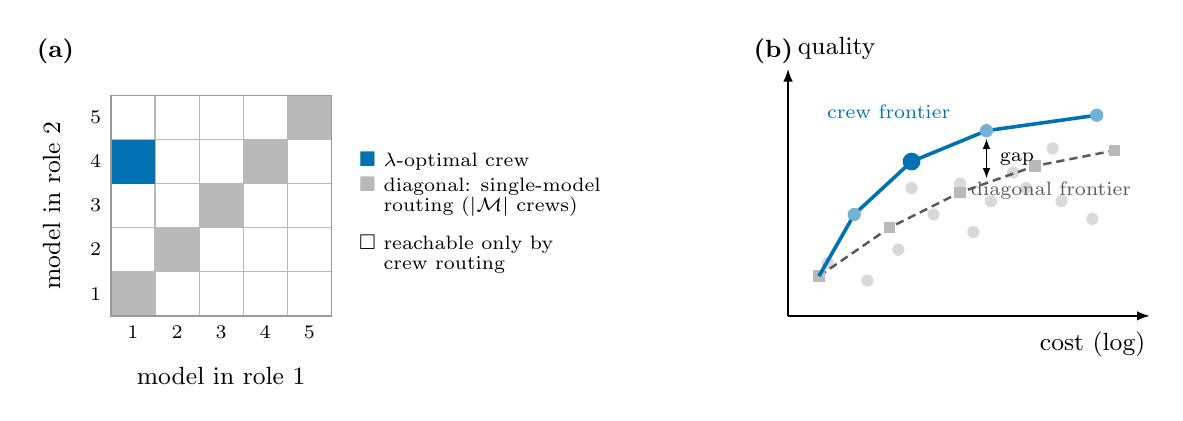
\begin{tikzpicture}[x=0.56cm,y=0.56cm,font=\small]
% (a) crew grid
\foreach \i in {0,...,4} \foreach \j in {0,...,4} {\draw[gray!55,fill=white] (\i,\j) rectangle ++(1,1);}
\foreach \i in {0,...,4} {\fill[gray!55] (\i,\i) rectangle ++(1,1); \draw[gray!55] (\i,\i) rectangle ++(1,1);}
\fill[ours] (0,3) rectangle ++(1,1);
\draw[gray!80,line width=0.5pt] (0,0) rectangle (5,5);
\foreach \i/\l in {0/1,1/2,2/3,3/4,4/5} {\node[font=\scriptsize,below] at (\i+0.5,0) {\l}; \node[font=\scriptsize,left] at (0,\i+0.5) {\l};}
\node[font=\small] at (2.5,-1.35) {model in role 1};
\node[font=\small,rotate=90] at (-1.35,2.5) {model in role 2};
\node[font=\bfseries\small,anchor=west] at (-1.9,6.0) {(a)};
\node[font=\scriptsize,anchor=west,align=left] at (5.4,3.5) {\textcolor{ours}{$\blacksquare$} $\lambda$-optimal crew};
\node[font=\scriptsize,anchor=west,align=left] at (5.4,2.7) {\textcolor{gray!55}{$\blacksquare$} diagonal: single-model\\[-1pt]\phantom{$\blacksquare$} routing ($|\mods|$ crews)};
\node[font=\scriptsize,anchor=west,align=left] at (5.4,1.4) {$\square$ reachable only by\\[-1pt]\phantom{$\square$} crew routing};
% (b) schematic frontier
\begin{scope}[xshift=8.6cm]
\draw[-{Latex[length=1.6mm]},line width=0.5pt] (0,0) -- (8.2,0) node[below left,font=\small,xshift=2pt,yshift=-2pt] {cost (log)};
\draw[-{Latex[length=1.6mm]},line width=0.5pt] (0,0) -- (0,5.6) node[above right,font=\small] {quality};
\foreach \x/\y in {0.9/1.2,2.5/1.5,1.8/0.8,3.3/2.3,4.2/1.9,5.4/2.9,6.2/2.6,3.9/3.0,5.1/3.25,6.9/2.2,2.8/2.9,4.6/2.6,6.0/3.8}
  {\fill[gray!30] (\x,\y) circle (2.2pt);}
\draw[gray!70!black,line width=0.9pt,dash pattern=on 3pt off 1.8pt] (0.7,0.9) -- (2.3,2.0) -- (3.9,2.8) -- (5.6,3.4) -- (7.4,3.75);
\foreach \x/\y in {0.7/0.9,2.3/2.0,3.9/2.8,5.6/3.4,7.4/3.75} {\fill[gray!55] (\x-0.13,\y-0.13) rectangle ++(0.26,0.26);}
\draw[ours,line width=1.3pt] (0.7,0.9) -- (1.5,2.3) -- (2.8,3.5) -- (4.5,4.2) -- (7.0,4.55);
\foreach \x/\y in {1.5/2.3,4.5/4.2,7.0/4.55} {\fill[ours!55] (\x,\y) circle (2.4pt);}
\fill[ours] (2.8,3.5) circle (3.2pt);
\draw[{Latex[length=1.3mm]}-{Latex[length=1.3mm]},line width=0.5pt] (4.5,3.12) -- (4.5,4.02);
\node[font=\scriptsize,anchor=west] at (4.58,3.55) {gap};
\node[font=\scriptsize,ours,anchor=south east] at (3.9,4.25) {crew frontier};
\node[font=\scriptsize,gray!70!black,anchor=north east] at (8.0,3.25) {diagonal frontier};
\node[font=\bfseries\small,anchor=west] at (-1.0,6.0) {(b)};
\end{scope}
\end{tikzpicture}
\caption{Crew routing generalises single-model routing (schematic, not data). (a) The crew space for $n=2$ roles and five candidate models per role, ordered by cost. A single-model router selects among the diagonal (grey); Pareto crewing searches all $|\mods|^n$ assignments, and its optimum (blue) may pair a low-cost model in one role with a stronger model in another. (b) The crew frontier is at least as high as the diagonal frontier (squares, dashed) at every budget, and strictly higher at some budgets whenever, at some price of quality, no single model is best in every role (\cref{prop:dominance}). \Cref{fig:crew-frontier} shows the measured counterpart.}
\label{fig:diagonal}
\end{figure}

\Cref{fig:headline} and \cref{tab:summary} summarise the effects we measure, each expressed as a cost-reduction factor at equal quality or a quality change at comparable cost. On real GitHub issues scored by two reviewers blind to configuration identity, the class-aware crew matches the best fixed crew's quality at $1.68\times$ lower cost (40\%), and improves on the best measured single-model (diagonal) policy by $+1.45$ review points, raising mergeable changes from 12 to 20 of 22, for \$0.025 more per issue. The best measured crew is class-dependent. On open-ended tasks it is off the diagonal: upgrading a subset of the low-cost crew's roles raises the mergeable rate from 0/8 to 8/8. On defect fixes it lies on the diagonal, and a uniformly low-cost crew is statistically indistinguishable from a uniformly frontier crew at $15.4\times$ lower cost. On DeepSWE, sequential search with a verifier of accuracy $r\ge0.8$ reaches the best configuration's success rate at 17--25$\times$ lower cost.

\begin{figure}[tbp]
\centering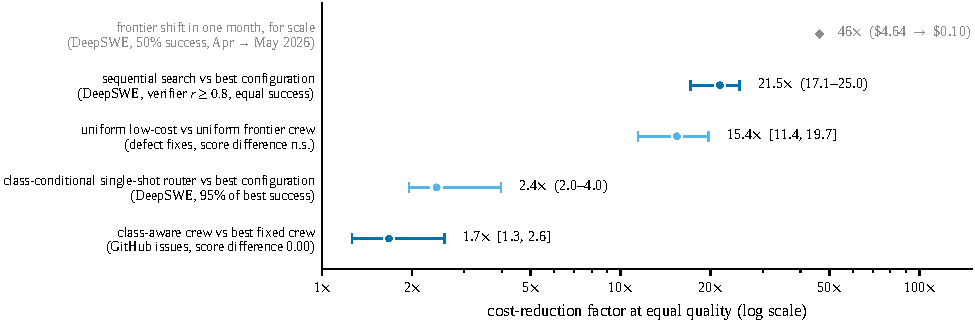
\includegraphics{fig-headline.pdf}
\caption{Cost-reduction factor at equal quality, per setting (log scale). GitHub-issue effects: ratio of mean costs with task-bootstrap 95\% CIs (22 and 14 issues); the quality difference is not significant in either. DeepSWE: range over verifier accuracies $r\in[0.8,1]$ (sequential search) and over target levels 90--98\% of the best configuration's success (single-shot). Grey: the shift of the frontier itself over one month, for scale.}
\label{fig:headline}
\end{figure}

\begin{table}[tbp]
\centering\small
\begin{tabularx}{\textwidth}{l>{\raggedright\arraybackslash}Xll}\toprule
setting & comparison & effect & quality\\\midrule
GitHub issues (22) & class-aware crew vs best fixed crew & 1.68$\times$ [1.26, 2.57] lower cost & score $\Delta=0.00$ [$-$0.75, +0.82]\\
GitHub issues (22) & class-aware crew vs best diagonal policy & mergeable 12 $\to$ 20, +\$0.025 & score $\Delta=+1.45$ [+0.64, +2.39]\\
Open-ended issues (8) & off-diagonal: checker upgrade only & mergeable 0\% $\to$ 100\% & score $\Delta=+4.00$ [+3.19, +4.94]\\
Defect fixes (14) & diagonal: uniform low-cost vs uniform frontier & 15.4$\times$ [11.4, 19.7] lower cost & score $\Delta=-0.29$ [$-$1.00, +0.46]\\
DeepSWE (111 tasks) & sequential search, $r\geq0.8$ & 17--25$\times$ lower cost & equal success (0.745)\\
DeepSWE (111 tasks) & single-shot class router & 2.4$\times$ lower cost & 95\% of best success\\
Unseen model families & credibility priors vs class means & closes 86\% of AIQ gap & $+0.153$ AIQ [0.145, 0.163]\\
DeepSWE frontier & Apr $\to$ May 2026, 50\% success & 46$\times$ lower cost & context\\
\bottomrule\end{tabularx}

\caption{Summary of results. Brackets: 95\% confidence intervals (task bootstrap); ranges: over verifier accuracy or target quality as stated. Diagonal policy: the same model in every role. AIQ: normalised area under the log-cost quality curve (\cref{sec:problem}).}
\label{tab:summary}
\end{table}

\paragraph{Contributions.}
\begin{itemize}
\item \textbf{Task-level multi-model routing with interacting roles, strictly generalising call-level single-model routing.} We define task-level routing, in which the decision is the crew and the reward and cost are whole-trajectory outcomes, and show that call-level routing is its restriction to role-additive surrogates, blind to interaction terms and to credit across calls (\cref{def:levels,prop:call}). Single-model routing is the further restriction to the diagonal of the crew space. The crew frontier weakly dominates the diagonal frontier for any quality function, any number of roles and any number of objectives; it strictly dominates it at some budget when the roles' leverage ratios straddle a non-negative operating multiplier and the diagonal contains a minimum-cost crew (\cref{prop:dominance}), and, for two roles, when one role compensates for the other's errors, even if one model has the highest additive score in both roles (\cref{prop:complement}); under role additivity the Lagrangian gap is non-decreasing in the number of roles (\cref{prop:gap}). The Lagrangian relaxation traces the exact frontier (\cref{prop:duality}), and the search over $\prod_s|\mods_s|$ crews reduces to $\sum_s|\mods_s|$ evaluations under role additivity and is $\eta$-optimal under interactions of range $\eta$ (\cref{prop:seat,prop:interact}).
\item \textbf{Approximate class sufficiency.} Task class captures nearly all of the achievable single-shot routing gain, which justifies a latent space conditioned on class rather than instance. Under conditional exchangeability of tasks within a class, the Bayes-optimal single-shot router depends on a task only through its class posterior, and if exchangeability holds up to $\varepsilon$ the class-conditional router is within $2\varepsilon$ of it (\cref{thm:class}). Across 21 evaluation matrices built from 34 benchmarks, the best instance-level feature family adds $+0.013\pm0.013$ AIQ over class identity (not significant) and $+0.006\pm0.002$ AIQ on the most precise split (significant, but small), whereas better class-level priors add $+0.07$ to $+0.15$ AIQ on held-out benchmark and model families; about 90\% of the apparent per-task headroom is run-to-run noise (\cref{sec:res-class}).
\item \textbf{Day-zero routing.} We define day-zero routing as routing a model before any outcome of that model has been observed. A two-level item-response model with guessing, fitted by marginal likelihood with Gauss--Hermite quadrature, with leaderboard aggregates as moment conditions and credibility blending from catalog metadata to pooled evidence to local outcomes (\cref{sec:priors}), closes 86\% of the gap between a class-mean router and the single-configuration hull on held-out model families ($+0.153$ AIQ) and gains $+0.072$ AIQ on held-out benchmark families (\cref{sec:res-priors}).
\item \textbf{Sequential Pareto search with correlated failures.} We define sequential Pareto search as adaptive purchase of further attempts on a task, driven by verification signals, evaluated against the single-configuration hull. We derive the verifier accuracy above which a two-stage search dominates the hull (\cref{thm:rstar}), show that its value falls with the covariance of failures across attempts (\cref{prop:retry}), and give an estimation-adjusted sufficient threshold $\hat r^\ast=0.65$ (\cref{prop:est}), an upper bound on the accuracy at which the learned policy's gain turns positive that is consistent with the observed transition between 0.6 and 0.7; a correlated Pandora-index policy gains $+0.172\pm0.022$ AIQ with an exact verifier (\cref{sec:res-seq}).
\item \textbf{The mechanism of heterogeneous crews.} The $\lambda$-optimal crew upgrades exactly the roles whose leverage ratio exceeds $\lambda$ (\cref{prop:rule}), and when one role compensates for another its leverage is proportional to the other's error rate on the class (\cref{prop:complement}; \cref{ex:verify}). On real issues the one upgrade measured on both classes, which changes a subset of the roles, has a leverage ratio of 59 review points per dollar on open-ended tasks and 0 on defect fixes, which places the best measured crew off the diagonal on one class and on it on the other (\cref{sec:trial}).
\end{itemize}
The method is implemented as the model-routing component of the CodeAF coding agent (\cref{sec:system}).

%======================================================================
\section{Problem formulation}
\label{sec:problem}
%======================================================================
\Cref{app:notation} collects the notation.


\begin{definition}[Roles, crews, routes]
Let $\seats=\{1,\dots,n\}$ be the roles of the agent (we also call them seats). Each model is reachable through a set of \emph{routes}: a pay-per-token API, a subscription with a quota, or a local runtime. Let $\mods$ be the finite set of \emph{configurations}: (model, route) pairs, with a reasoning-effort setting where the model has one; we write $m\in\mods$ and call $m$ a model when the route is immaterial. For role $s$, the candidate set $\mods_s\subseteq\mods$ consists of the admissible configurations, those whose model is in the allowed set and is able to hold the role. A \emph{crew} is a tuple $\crew=(m_1,\dots,m_n)\in\mods_1\times\dots\times\mods_n$; we write $\crew_{-s}$ for the assignment of all roles other than $s$ and $(\crew_{-s},m_s')$ for the crew with role $s$ reassigned.
\end{definition}

\begin{definition}[Diagonal]
Let $\mods_\cap=\bigcap_{s}\mods_s$ be the (model, route) pairs admissible in every role. The \emph{diagonal} of the crew space is the set of uniform crews $\mathcal D=\{(m,\dots,m):m\in\mods_\cap\}$. A single-model router, which sends every call of a task to one model, selects from $\mathcal D$.
\end{definition}
When every role admits the same $|\mods|$ candidates, the diagonal holds $|\mods|$ of the $|\mods|^n$ crews, a fraction $|\mods|^{1-n}$ that vanishes exponentially in the number of roles: 20 candidates and three roles give 20 uniform crews out of 8{,}000.

\begin{definition}[Tasks and classes]
A task $t$ has a description $x_t$ and a class $c_t\in\cls$. We use three classes, \emph{bug-fix}, \emph{open-ended} and \emph{other}, where open-ended covers feature, refactor, documentation and design work. A classifier returns a class posterior $\psi(c\mid x)$, calibrated so that $\psi(c\mid x)\approx\Pr(c_t=c\mid x_t=x)$.
\end{definition}

\begin{definition}[Call profile and route-aware marginal cost]
Role $s$ on a class-$c$ task has a \emph{call profile}: the expected number of calls $N_s(c)$ and input and output tokens per call $T^{\rm in}_s(c)$, $T^{\rm out}_s(c)$. A configuration $m$ with model $\mu$ and route $\nu$ has marginal token prices $p^{\rm in}(m)$, $p^{\rm out}(m)$: the list price on an API route; zero on a local route; on a subscription with remaining quota fraction $\phi$, the list price times $h(\phi)$, with $h$ non-increasing, $h(\phi)=0$ for $\phi\ge\phi_0$ and $h(0)=1$. The marginal cost of role $s$ and of the crew are
\begin{equation}
c_s(m_s;c)=N_s(c)\big(T^{\rm in}_s(c)\,p^{\rm in}(m_s)+T^{\rm out}_s(c)\,p^{\rm out}(m_s)\big),\qquad C(\crew;c)=\sum_{s=1}^{n}c_s(m_s;c).
\label{eq:cost}
\end{equation}
\end{definition}

Under the route-aware cost the same model can be cheap on one route and expensive on another; in particular, a subscription has zero marginal cost until its quota runs low. Cost is additive over roles by construction; quality in general is not.

Let $Q(\crew;c)\in[0,1]$ be the expected quality of crew $\crew$ on class $c$ (a success probability, or a review score divided by 10). $Q$ is an arbitrary function of the full tuple, so interactions between roles are allowed; where a result needs more structure we state it as an assumption. A \emph{policy} maps a task to a distribution over admissible crews. For a budget $B$ per task, the problem is
\begin{equation}
F(B)=\max_{\pi}\ \E_{t}\,\E_{\crew\sim\pi(t)}\,Q(\crew;c_t)\quad\text{s.t.}\quad \E_t\,\E_{\crew\sim\pi(t)}\,C(\crew;c_t)\le B.
\label{eq:primal}
\end{equation}
for $B\ge B_{\min}:=\E_t\min_\crew C(\crew;c_t)$, below which no policy is feasible.

\begin{proposition}[The Lagrangian sweep traces the hull]
\label{prop:duality}
For the finite set $\mods_1\times\dots\times\mods_n$ of admissible crews, any $n$, any $Q$, and randomized policies, $F$ is concave, non-decreasing and piecewise linear, and
\[
F(B)=\min_{\lambda\ge0}\Big\{\lambda B+\E_t\max_{\crew}\big[Q(\crew;c_t)-\lambda\,C(\crew;c_t)\big]\Big\}.
\]
Every vertex of $F$ is attained by the deterministic policy $\crew_\lambda(t)=\argmax_{\crew}\,Q(\crew;c_t)-\lambda C(\crew;c_t)$ for some $\lambda$, and every point between two vertices by mixing the two.
\end{proposition}
The proof (\cref{app:proofs}) is linear-programming duality: \eqref{eq:primal} is a linear program over the simplex of crew distributions per class. Consequently a single scalar $\lambda$ indexes every Pareto-optimal policy; its units are quality per dollar, the rate at which quality is traded for cost.


\begin{definition}[AIQ]
For a policy family with frontier $F_\pi$, the \emph{area under the log-cost quality curve} over a budget range $[B_{\rm lo},B_{\rm hi}]$ is
\begin{equation}
\AIQ(\pi)=\frac{1}{\log(B_{\rm hi}/B_{\rm lo})}\int_{\log B_{\rm lo}}^{\log B_{\rm hi}} F_\pi(e^u)\dd u ,
\label{eq:aiq}
\end{equation}
with $F_\pi(B)=0$ below the policy's cheapest point. The range is fixed by the cheapest and the most expensive single configuration on the test set, and $F_\pi$ is the upper concave non-decreasing envelope of the realised points in linear cost $B$ (the frontier of randomised policies).
\end{definition}
The log scale weights each doubling of the budget equally; the price of capability spans two to three orders of magnitude, so a linear scale would score only the expensive end. AIQ is invariant to a common rescaling of all prices together with the range.

\begin{definition}[Knee]
Plot the frontier $F$ (concave in linear cost $B$) against $u=\log B$ over $[u_0,u_1]$, with endpoint values $F_0=F(e^{u_0})$ and $F_1=F(e^{u_1})$. The \emph{knee} is the point farthest above the chord (the smallest such $u$ in case of ties),
\begin{equation}
u^\star=\min\argmax_{u\in[u_0,u_1]}\ \Big[F(e^u)-F_0-(F_1-F_0)\frac{u-u_0}{u_1-u_0}\Big],
\label{eq:knee}
\end{equation}
the Kneedle point \cite{satopaa2011}. The default operating point is $\lambda_{\rm knee}=\bar d/e^{u^\star}$ with chord slope $\bar d=(F_1-F_0)/(u_1-u_0)$.
\end{definition}

\begin{proposition}[Invariance of the knee]
\label{prop:knee}
The knee is unchanged by a common rescaling of all prices, $B\mapsto\alpha B$ with $\alpha>0$, and by a shift of quality $F\mapsto F+\beta_0$. If the knee is interior, $u_0<u^\star<u_1$, then $\partial_u^+F(e^{u^\star})\le\bar d\le\partial_u^-F(e^{u^\star})$; hence $\lambda_{\rm knee}=\bar d/e^{u^\star}$ is a supporting multiplier of $F$ at $B=e^{u^\star}$. The knee can also lie at an endpoint, where this slope condition need not hold.
\end{proposition}
Market-wide price cuts move the default crew only when they change \emph{relative} prices.

\subsection{Task-level routing and role interactions}
\label{sec:levels}

Write $L_\lambda(\crew;c)=Q(\crew;c)-\lambda C(\crew;c)$ for the Lagrangian of \cref{prop:duality}.

\begin{definition}[Call-level and task-level routing]
\label{def:levels}
A task is executed as a trajectory of calls $k=1,\dots,K$; call $k$ is made by role $s(k)$ with the model assigned to that role. A \emph{call-level} router chooses the model of each call and maximises a per-call objective $r_k(m)-\lambda C_k(m)$, with $C_k$ the call's cost, in which the reward $r_k$ is credited to call $k$ alone. A \emph{task-level} router chooses the crew $\crew$ for the whole task and maximises $L_\lambda(\crew;c)$, where $Q$ and $C$ are the quality and cost of the whole trajectory.
\end{definition}

\begin{definition}[Interaction decomposition]
\label{def:interact}
Fix an admissible reference crew $\crew^0\in\prod_s\mods_s$. Every $Q$ can be written as
\begin{equation}
Q(\crew;c)=q_0(c)+\sum_{s=1}^n q_s(m_s;c)+\sum_{s<t}I_{st}(m_s,m_t;c)+R(\crew;c),
\label{eq:interact}
\end{equation}
with baseline $q_0(c)=Q(\crew^0;c)$, main effects $q_s(m;c)=Q((\crew^0_{-s},m);c)-Q(\crew^0;c)$, pairwise interactions
\[
I_{st}(m_s,m_t;c)=Q\big((\crew^0_{-st},m_s,m_t);c\big)-Q(\crew^0;c)-q_s(m_s;c)-q_t(m_t;c),
\]
where $(\crew^0_{-st},m_s,m_t)$ is the reference crew with roles $s$ and $t$ reassigned, and a higher-order remainder $R$ of range $\eta_R=\max R-\min R$. Roles $s$ and $t$ \emph{interact} (relative to $\crew^0$) if $I_{st}\not\equiv0$; for $n\ge3$ this can depend on the reference, because a three-way term can appear in $I_{st}$ at some references and not at others.
\end{definition}

\begin{assumption}[Role additivity]
\label{ass:add}
$I_{st}\equiv0$ for all $s<t$ and $R\equiv0$, so that $Q(\crew;c)=q_0(c)+\sum_{s=1}^n\delta_s(m_s;c)$ with $\delta_s=q_s$.
\end{assumption}

\begin{assumption}[Monotonicity in roles]
\label{ass:mono}
Each $\mods_s$ carries a partial order $\preceq_s$ (an \emph{upgrade} relation) such that $m_s\preceq_s m_s'$ implies $Q((\crew_{-s},m_s');c)\ge Q(\crew;c)$ for every $\crew_{-s}$ and $c$.
\end{assumption}

\begin{proposition}[Call-level routing is a restriction]
\label{prop:call}
Suppose each call's reward and cost depend only on its role, its model and the class (an assumption that excludes per-call credit depending on the call's context), and let $\bar r_s(m;c)$ and $c_s(m;c)$ be the expected reward and cost credited to role $s$ per task.
\begin{enumerate}[label=(\roman*),leftmargin=*]
\item The call-level router selects the crew $\hat\crew=\argmax_\crew\sum_s[\bar r_s(m_s;c)-\lambda c_s(m_s;c)]$, the maximiser of a role-additive surrogate. Since $\hat\crew$ is admissible for the task-level problem, $\max_\crew L_\lambda(\crew;c)\ge L_\lambda(\hat\crew;c)$.
\item The call-level choice is unchanged if the interaction terms $I_{st}$ and $R$ of $Q$ are changed arbitrarily: call-level routing cannot represent role interactions.
\item If the per-call credit recovers the main effects, $\bar r_s=q_s$, then $\max_\crew L_\lambda-L_\lambda(\hat\crew)\le\eta$, where $\eta$ is the range of $\sum_{s<t}I_{st}+R$, and the two coincide under \cref{ass:add}.
\end{enumerate}
\end{proposition}
Part (ii) is the credit-assignment problem in its simplest form. A call's contribution to the task outcome depends on the other calls of the trajectory: a defect introduced in one role is worth more to a later role that can catch it. A reward credited to a single call can express only that call's main effect.

\paragraph{Latent, class-conditional parameterisation.} Main effects and interactions are not estimated crew by crew. They are functions of latent model abilities and of the distribution of task difficulty within the class: $Q(\crew;c)=\E_{z\sim G_c}\,f(\theta_{m_1},\dots,\theta_{m_n},z)$, with the item-response model of \cref{sec:priors} for $\theta$ and $z$. Conditioning on the class rather than the task instance is justified by approximate class sufficiency (\cref{thm:class}): the instance adds at most about 0.01 AIQ of routing value beyond its class (\cref{sec:res-class}). The same latent model, extended with two random effects, describes repeated attempts: an attempt of configuration $m$ on task $t$ succeeds with probability $\sigma(\ell_m-\kappa_m\tau z_t+u_{t,{\rm base}(m)}+e_{tm})$, with $u_{t,{\rm base}}\sim\mathcal N(0,\omega_{\rm base}^2)$ shared by the configurations of one base model and $e_{tm}\sim\mathcal N(0,\omega_m^2)$ specific to the configuration, so failures are correlated across configurations through the shared difficulty $z_t$ and across configurations of one base model through $u$, and a retry of the same configuration repeats its task-specific effect $e_{tm}$ (\cref{prop:retry}).

\subsection{Crews versus single models}
\label{sec:diagonal}

Write $F_{\rm crew}$ for the frontier \eqref{eq:primal} over all crews and $F_{\rm diag}$ for the frontier over the diagonal $\mathcal D$ only. Under \cref{ass:add}, $L_\lambda(\crew;c)=q_0(c)+\sum_s g_s(m_s)$ with the \emph{role utility} $g_s(m)=\delta_s(m;c)-\lambda c_s(m;c)$. For two models $a,b\in\mods_\cap$ with $c_s(b;c)>c_s(a;c)$ in every role, the \emph{leverage ratio} of upgrading role $s$ from $a$ to $b$ is $\Lambda_s=\big(\delta_s(b;c)-\delta_s(a;c)\big)/\big(c_s(b;c)-c_s(a;c)\big)$, the quality gained per unit of added cost; under \cref{ass:add} it equals $\Lambda_s(c)$ of \cref{def:leverage} for any crew.

\begin{proposition}[Crew dominance]
\label{prop:dominance}
Fix a class $c$.
\begin{enumerate}[label=(\roman*),leftmargin=*]
\item \emph{Weak dominance.} For any $Q$, any $n$ and every $\lambda\ge0$, $\max_{\crew}L_\lambda(\crew;c)\ge\max_{\crew\in\mathcal D}L_\lambda(\crew;c)$, and $F_{\rm crew}(B)\ge F_{\rm diag}(B)$ for every budget $B$ at which $F_{\rm diag}$ is feasible.
\item \emph{Strictness.} Under \cref{ass:add}, $\max_{\crew}L_\lambda>\max_{\crew\in\mathcal D}L_\lambda$ if and only if no $m\in\mods_\cap$ maximises every $g_s$ over $\mods_s$. In particular, if every role chooses between two models $a$ and $b$ as above ($\mods_s=\{a,b\}$), the $\lambda$-optimal crew is off the diagonal, and its Lagrangian value strictly exceeds that of both uniform crews, whenever
\[
\min_s\Lambda_s<\lambda<\max_s\Lambda_s .
\]
\item \emph{Strict frontier gap.} If $\max_{\crew}L_\lambda>\max_{\crew\in\mathcal D}L_\lambda$ at some $\lambda\ge0$, then $F_{\rm crew}(B)>F_{\rm diag}(B)$ for some budget $B$, with the convention $F_{\rm diag}(B)=-\infty$ where no diagonal policy is feasible. If $\mathcal D$ contains a minimum-cost crew (for instance $c_s(b;c)>c_s(a;c)$ for all $s$ in (ii)), the budget can be taken with $F_{\rm diag}(B)$ finite.
\end{enumerate}
For a distribution over classes, (i) holds for the population frontier, and (iii) holds whenever the condition of (ii) is met on a class of positive probability.
\end{proposition}

Part (i) holds because the diagonal is a subset of the crew space. Part (ii) says when the inclusion is strict: the roles must disagree about which model is worth its cost. With two models, the roles with leverage above the operating multiplier take the stronger model and the others the cheaper one, so any spread of leverage ratios across roles that contains some $\lambda\ge0$, i.e.\ $\max_s\Lambda_s>\max\{0,\min_s\Lambda_s\}$, yields a heterogeneous crew that no single-model router can express. The frontier gap it creates is strict only at some budgets; at others the two frontiers can coincide. \Cref{sec:leverage} gives the mechanism that produces such a spread, and \cref{sec:trial} measures it.

\paragraph{Compensating roles.} \Cref{prop:dominance}(ii) needs role additivity. With interactions, the optimal crew can leave the diagonal for a different reason: the value of one role can depend on the model in another. Fix all roles except $s$ and $t$, and two models $a,b$ admissible in both with $c_s(b)>c_s(a)$ and $c_t(b)>c_t(a)$; write $Q(x,y)$ for the crew with $x$ in role $s$ and $y$ in role $t$, $\Delta c_r=c_r(b)-c_r(a)$, and the \emph{conditional leverage ratios}
\[
\Lambda_{t\mid x}=\frac{Q(x,b)-Q(x,a)}{\Delta c_t},\qquad \Lambda_{s\mid y}=\frac{Q(b,y)-Q(a,y)}{\Delta c_s},
\]
the leverage of upgrading one role given the model in the other. Role $t$ \emph{compensates} for role $s$ if upgrading $t$ is worth more when $s$ holds the weaker model, $\Lambda_{t\mid a}>\Lambda_{t\mid b}$. Equivalently the pairwise interaction contrast is positive,
\[
Q(a,b)+Q(b,a)-Q(a,a)-Q(b,b)=\Delta c_t\big(\Lambda_{t\mid a}-\Lambda_{t\mid b}\big)=\Delta c_s\big(\Lambda_{s\mid a}-\Lambda_{s\mid b}\big)>0,
\]
so the relation is symmetric. In standard terminology the two roles' strengths are \emph{substitutes}: $Q$ is submodular in $(m_s,m_t)$ under the order $a\prec b$; equivalently the error of role $s$ and the strength of role $t$ are complements. When the gain from upgrading role $t$ grows with the error rate of role $s$, and $a$ errs more than $b$ in role $s$, the pair is compensating; \cref{ex:verify} gives a construction.

\begin{proposition}[Compensating roles]
\label{prop:complement}
In the setting above, where ``uniform'' and ``off the diagonal'' refer to the pair $(s,t)$ with the other roles fixed (for $n=2$ this is the diagonal $\mathcal D$):
\begin{enumerate}[label=(\roman*),leftmargin=*]
\item If $\Lambda_{s\mid b}<\lambda<\Lambda_{t\mid a}$, the $\lambda$-optimal crew over $\{a,b\}^2$ is off the diagonal, and its Lagrangian value strictly exceeds that of both uniform crews.
\item Consider the role-additive surrogate whose main effects are measured against the uniform strong crew: it assigns $b$ to role $s$ if and only if $\Lambda_{s\mid b}>\lambda$, and to role $t$ if and only if $\Lambda_{t\mid b}>\lambda$. If $b$ has the higher additive score in both roles, $\Lambda_{s\mid b},\Lambda_{t\mid b}>0$, then for every $\lambda$ with $\max\{\Lambda_{s\mid b},\Lambda_{t\mid b}\}<\lambda<\Lambda_{t\mid a}$ the surrogate selects the uniform crew $(a,a)$, whereas the $\lambda$-optimal crew is off the diagonal and strictly better. For a compensating pair this interval is non-empty whenever $\Lambda_{s\mid b}<\Lambda_{t\mid a}$, including when the additive leverage ratios do not straddle $\lambda$.
\end{enumerate}
\end{proposition}
Under additivity, \cref{prop:dominance}(ii) requires the roles' leverage ratios to straddle $\lambda$. Compensation produces an off-diagonal optimum even when both additive ratios lie below $\lambda$, so that an additive analysis would keep the crew uniform and low-cost. For $n=2$, \cref{prop:dominance}(iii) turns the strict Lagrangian gap of \cref{prop:complement}(i) into a strict frontier gap at some budget, and since $(a,a)$ is the minimum-cost crew that budget has a finite diagonal frontier. For $n>2$ the result compares the pair's crews with the two pair-uniform crews at fixed other roles, which are not in $\mathcal D$; a fully uniform crew can still beat every crew of the pair, so the statement does not by itself give a gap to $F_{\rm diag}$.

\begin{proposition}[The gap grows with the number of roles]
\label{prop:gap}
Under \cref{ass:add}, with a common candidate set for all roles, let $G_n(\lambda)=\max_{\crew}L_\lambda-\max_{\crew\in\mathcal D}L_\lambda\ge0$ for a crew of roles $1,\dots,n$. Adding a role never decreases the gap: $G_{n+1}(\lambda)\ge G_n(\lambda)$ for every $\lambda$.
\end{proposition}

\paragraph{More than two objectives.} The formulation extends to $d$ objectives. Let $\mathbf o(\crew;c)\in\R^d$ collect quality and the negated resources to be minimised (cost, tokens, and latency where roles run sequentially, so that it adds over roles); a crew is Pareto-optimal if no other crew is at least as good in every coordinate and better in one. The scalarisation $\max_\crew\langle w,\mathbf o(\crew;c)\rangle$ with $w\in\R^d_{>0}$ traces the supported Pareto points ($w\ge0$ gives weakly Pareto-optimal points), which randomised policies fill in by mixing at most $d$ deterministic crews; with $d=2$ and $w=(1,\lambda)$ it is $L_\lambda$. Because the diagonal is a subset of the crew space, every vector attainable by a diagonal policy is attainable by a crew policy, so part (i) of \cref{prop:dominance} holds for any $d$. When every objective is additive over roles, the characterisation in (ii) holds with $g_s(m)=\langle w,\mathbf o_s(m;c)\rangle$, and (iii) becomes: a strict support-function gap in direction $w$ implies an objective vector of some crew policy that no diagonal policy weakly dominates. All experiments in this paper use $d=2$ (quality and cost); we make no empirical claim about other objectives.

%======================================================================
\section{Method}
\label{sec:method}
%======================================================================

\Cref{fig:pipeline} shows the router. A task is classified; the candidate set is the allowed models reachable through available routes; each (class, role, model) receives a quality prior and each role a route-aware cost; the crew maximising $Q-\lambda C$ is chosen; a sequential layer decides whether to escalate after a verifier signal; and a pacing loop adjusts $\lambda$ against a budget.

\begin{figure}[tbp]
\centering
\resizebox{\textwidth}{!}{%
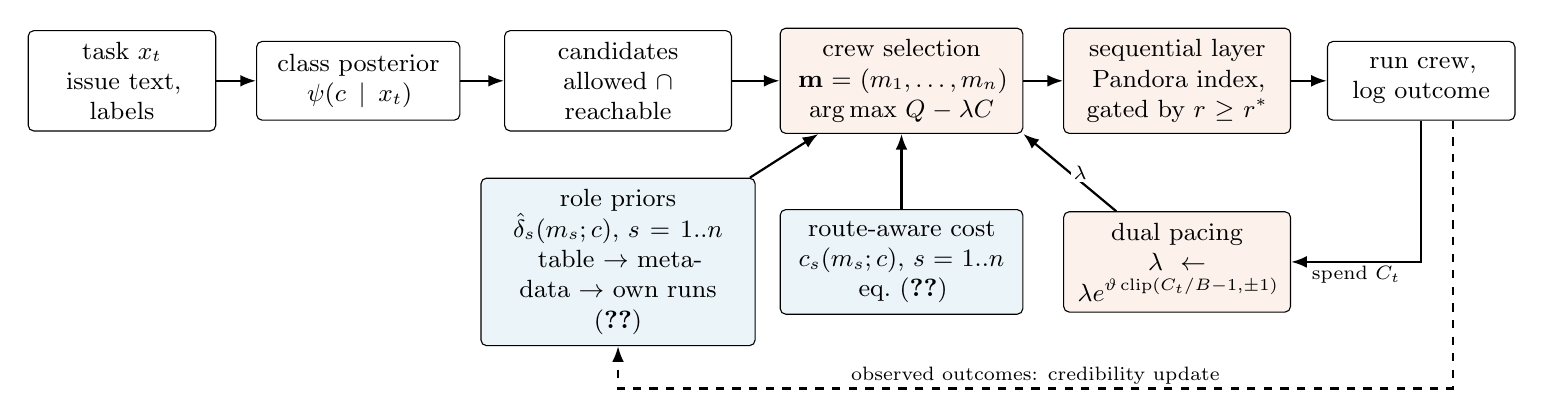
\begin{tikzpicture}[x=1cm,y=1cm,
  box/.style={draw,rounded corners=2pt,inner sep=4pt,font=\small,align=center,minimum height=10mm,fill=white},
  prior/.style={box,fill=ours!8},
  dec/.style={box,fill=chk!8},
  arr/.style={-{Latex[length=2mm]},thick},
  lbl/.style={font=\scriptsize,fill=white,inner sep=1pt}]
\node[box,text width=2.1cm] (task) at (0,0) {task $x_t$\\issue text, labels};
\node[box,text width=2.3cm] (clf) at (3.0,0) {class posterior\\$\psi(c\mid x_t)$};
\node[box,text width=2.6cm] (cand) at (6.3,0) {candidates\\allowed $\cap$\\reachable};
\node[prior,text width=3.2cm] (prior) at (6.3,-2.3) {role priors $\hat\delta_s(m_s;c)$, $s=1..n$\\table $\to$ metadata $\to$ own runs\\(\cref{sec:priors})};
\node[prior,text width=2.8cm] (cost) at (9.9,-2.3) {route-aware cost\\$c_s(m_s;c)$, $s=1..n$\\eq.~\eqref{eq:cost}};
\node[dec,text width=2.8cm] (sel) at (9.9,0) {crew selection\\$\crew=(m_1,\dots,m_n)$\\$\argmax\,Q-\lambda C$};
\node[dec,text width=2.6cm] (seq) at (13.4,0) {sequential layer\\Pandora index,\\gated by $r\ge r^\ast$};
\node[box,text width=2.1cm] (run) at (16.5,0) {run crew,\\log outcome};
\node[dec,text width=2.6cm] (pace) at (13.4,-2.3) {dual pacing\\$\lambda\leftarrow\lambda e^{\vartheta\,\mathrm{clip}(C_t/B-1,\pm1)}$};
\draw[arr] (task) -- (clf);
\draw[arr] (clf) -- (cand);
\draw[arr] (cand) -- (sel);
\draw[arr] (prior) -- (sel);
\draw[arr] (cost) -- (sel);
\draw[arr] (sel) -- (seq);
\draw[arr] (seq) -- (run);
\draw[arr] (pace) -- node[lbl,right]{$\lambda$} (sel.south east);
\draw[arr] (run.south) |- node[lbl,pos=0.75,below]{spend $C_t$} (pace.east);
\draw[arr,dashed] (run.south) ++(0.4,0) -- ++(0,-3.4) -| node[lbl,pos=0.25,above]{observed outcomes: credibility update} (prior.south);
\end{tikzpicture}}
\caption{The per-task crew router. Blue: the evidence layer, which turns public benchmarks, catalog metadata and an install's own outcomes into a quality prior per (class, role, model) for roles $s=1,\dots,n$. Orange: the decision layer. Crew selection searches the full crew space, not only its diagonal; under role additivity the whole path is a table lookup and $\sum_s|\mods_s|$ evaluations (\cref{prop:seat}).}
\label{fig:pipeline}
\end{figure}

\subsection{Classification}
The classifier maps issue text and labels to $\psi(c\mid x)$. It is a pruned multinomial logistic regression on hashed word uni- and bi-grams with at most 2{,}000 non-zero weights per class stored as 8-bit integers, calibrated by a temperature and a floor mixed with the class prior. Structural signals (issue labels, stack traces, imperative verbs such as \emph{add}, \emph{support}, \emph{refactor}) enter as additional features. An uncertain task is routed as open-ended: on the real-issue trial (\cref{sec:trial}) that choice costs \$0.06 on a defect fix, while it is worth 8 of 8 mergeable changes on open-ended work.

\subsection{Priors: hierarchical IRT with credibility}
\label{sec:priors}

The quality prior must exist for every (class, model) pair on the day a model appears. We build it in two levels.

\paragraph{Level 1: cross-benchmark ability.}
Let $u$ index \emph{units} (a benchmark, or a benchmark subset with at least 30 training tasks) and $m$ a candidate (a model, or a model at a reasoning-effort setting). With cell means $\bar y_{um}$ and weights $w_{um}=\min(n_{um},200)$,
\begin{equation}
\zeta_{um}=\alpha_u^\top\theta_m+\beta_u,\qquad
\theta_m=\theta_{\mathrm{base}(m)}+\gamma_{\mathrm{effort}(m)}+\varepsilon_m,\qquad
\theta_{\mathrm{base}}\sim\mathcal N(Wx_{\mathrm{base}},I),\ \ \varepsilon_m\sim\mathcal N(0,0.3^2 I),
\label{eq:level1}
\end{equation}
with $\theta_m\in\R^3$ and $x$ the catalog metadata vector (log prices, release date, context length, open weights, reasoning flag, provider, missing-value flags). The loss is $\sum_{um}w_{um}\,\mathrm{BCE}(\bar y_{um},\sigma(\zeta_{um}))$ plus the Gaussian priors, minimised by L-BFGS. A model without a single benchmark row is placed by its metadata through $W$.

\paragraph{Aggregates as moment conditions.}
A new model usually has only published leaderboard numbers. A published score $S_{bm}$ on benchmark $b$ is the population mean of the per-task success probability, which gives one moment condition per (benchmark, model):
\begin{equation}
\E_{t\in b}\big[\Pr(y_{tm}=1\mid\theta_m,z_t)\big]=S_{bm}.
\label{eq:llp}
\end{equation}
We impose \eqref{eq:llp} as a penalty $n_{\rm llp}\,\mathrm{BCE}\big(S_{bm},\ \overline{P}_{bm}(\theta_m)\big)$ with $n_{\rm llp}=30$, the learning-from-label-proportions form of the constraint \cite{quadrianto2009}; aggregate cells enter Level 1 with weight 50.

\paragraph{Level 2: within-benchmark IRT with guessing.}
Within benchmark $b$, tasks in unit $u$ are exchangeable with latent difficulty $z_t\sim\mathcal N(0,1)$ and
\begin{equation}
\Pr(y_{tm}=1\mid z_t)=g_u+(1-g_u)\,\sigma\!\big(\ell_{um}-\kappa_m\tau_u z_t\big),\qquad
\ell_{um}\sim\mathcal N\big(\ell^0_{um},\varsigma_b^2\big),
\label{eq:irt}
\end{equation}
where $g_u$ is a guessing floor (binary units only), $\tau_u$ the spread of difficulty in the unit, $\kappa_m$ a per-model discrimination with $\log\kappa_m\sim\mathcal N(0,0.3^2)$, and $\ell^0_{um}=\zeta_{um}\sqrt{1+\pi\tau_u^2\kappa_m^2/8}$ the Level-1 prediction mapped to the conditional scale (here $\pi$ is the constant; the mapping inverts the probit approximation to the marginal logistic and ignores the guessing floor, so it is approximate on binary units). This is the three-parameter logistic model \cite{birnbaum1968,lord1980} with a hierarchical prior on the item-side intercepts.

\paragraph{Marginal likelihood by quadrature.}
The difficulty is integrated out on a $G$-point Gauss--Hermite grid $\{(z_g,\omega_g)\}$ \cite{bock1981,abramowitz1964}:
\begin{equation}
\log L=\sum_t\log\sum_{g=1}^{G}\omega_g\prod_{m\in\mathrm{obs}(t)}P_{um}(z_g)^{y_{tm}}\big(1-P_{um}(z_g)\big)^{1-y_{tm}}+\log p(\ell,\kappa,\tau,g).
\label{eq:ghq}
\end{equation}
With $G=41$ the rule integrates polynomials of degree 81 in $z$ exactly; the integrand is smooth and bounded, and the quadrature error is below the optimiser tolerance. Fractional outcomes (means over repeats, judge scores) use the Bernoulli quasi-likelihood, which is consistent for $\E[y]$.

\paragraph{Credibility blending.}
The prior scale $\varsigma_b$ decides how far a cell follows its own data. Under \eqref{eq:irt} and a Laplace approximation, the posterior mean of $\ell_{um}$ is
\begin{equation}
\hat\ell_{um}=Z_{um}\,\tilde\ell_{um}+(1-Z_{um})\,\ell^0_{um},\qquad Z_{um}=\frac{n_{um}\bar I_{um}}{n_{um}\bar I_{um}+\varsigma_b^{-2}},
\label{eq:cred}
\end{equation}
where $\tilde\ell_{um}$ is the cell's own maximum-likelihood value and $\bar I_{um}$ the mean observed information per task at $\tilde\ell_{um}$ (\cref{prop:cred}). This is B\"uhlmann credibility \cite{buhlmann1967,buhlmann2005} with credibility constant $n_0=1/(\varsigma_b^2\bar I)$. The deployed prior nests it three times: catalog metadata $\to$ pooled benchmark evidence $\to$ the install's own outcomes, each level shrinking toward the one above with its own $Z$ (approximately; \cref{prop:cred}). The scale $\varsigma_b$ is initialised by a moment estimate on data-rich cells and then chosen on validation likelihood from $\{0.3,1.2\}$ (\cref{app:hyper}).

\paragraph{A new model after $K$ anchors.}
When a model is run on $K$ anchor tasks, its posterior variance is $v_K=(\varsigma_b^{-2}+\sum_{t\le K}I_t)^{-1}$ and the expected loss of routing on the posterior mean shrinks as $v_K$ (\cref{prop:anchor}). We draw anchors uniformly at random from the class (\cref{sec:res-priors} explains why random beats D-optimal selection on real data).

\subsection{Crew selection}
\label{sec:select}

For a class $c$ and multiplier $\lambda$ the router maximises $L_\lambda(\crew;c)=Q(\crew;c)-\lambda C(\crew;c)$ over $\mods_1\times\dots\times\mods_n$, the full crew space rather than its diagonal. Exhaustive search evaluates $\prod_{s}|\mods_s|$ crews, which grows exponentially in $n$; \cref{ass:add} makes the search linear in $n$.

The quality prior is stored per (class, role, model) as the estimates $\hat\delta_s(m;c)$ of \cref{ass:add}; \cref{sec:trial} measures role effects directly on real issues.

\begin{proposition}[Per-role decomposition]
\label{prop:seat}
Under \cref{ass:add} and \eqref{eq:cost}, for any $n$ and $\lambda\ge0$,
\[
\argmax_{\crew}\ L_\lambda(\crew;c)=\Big(\argmax_{m_s\in\mods_s}\ \delta_s(m_s;c)-\lambda\,c_s(m_s;c)\Big)_{s=1,\dots,n},
\]
computed with $\sum_s|\mods_s|$ evaluations instead of $\prod_s|\mods_s|$.
\end{proposition}

\begin{proposition}[Interactions of bounded range]
\label{prop:interact}
Let $Q=Q_{\rm add}+Q_{\rm int}$ with $Q_{\rm add}$ additive as in \cref{ass:add} and $\eta=\max_{\crew}Q_{\rm int}(\crew;c)-\min_{\crew}Q_{\rm int}(\crew;c)$. The per-role solution $\hat\crew$ of $Q_{\rm add}-\lambda C$ satisfies $L_\lambda(\hat\crew;c)\ge\max_\crew L_\lambda(\crew;c)-\eta$. Cyclic coordinate ascent on $L_\lambda$ started at $\hat\crew$, reassigning one role at a time, costs $\sum_s|\mods_s|$ evaluations of $Q$ per sweep, never decreases $L_\lambda$, and terminates after finitely many sweeps at a role-wise optimum, a crew that no single-role reassignment improves. Under \cref{ass:add} the first sweep reaches the global optimum and the second confirms it.
\end{proposition}

With $n=3$ roles and a few hundred (model, route) pairs per role, the decomposition replaces $10^{7}$ crew evaluations by $10^{3}$. The default operating point is $\lambda_{\rm knee}$; $\lambda\to0$ selects the highest-quality crew and the largest $\lambda$ on the class's hull grid the cheapest.

\subsection{Sequential search with a noisy verifier}
\label{sec:seq}

After an attempt, a verifier (a verdict from another role, the repository's tests, or a user's acceptance) returns a signal $v\in\{\text{pass},\text{fail}\}$ with $\Pr(v=y)=r$. The sequential layer decides whether to accept the best answer so far or to buy another attempt.

\paragraph{Within-task posterior.}
The task's latent $z_t$ is kept as a posterior on the quadrature grid and updated by each signal; a persistent task$\times$configuration effect $e_{tm}\sim\mathcal N(0,\omega_m^2)$ makes a retry of a configuration that just failed less likely to pass than a fresh configuration of equal strength. On the DeepSWE trials the fitted spreads are $\tau\approx1.6$, $\omega_m\approx1.5$ (median) and $\omega_{\rm base}\approx0.2$, so most of the stickiness of failure is at the (task, configuration) level.

\paragraph{Reservation index.}
Let $X_m$ be the posterior probability that configuration $m$'s answer is correct after its own signal. The index $\sigma_m$ solves
\begin{equation}
\E\big[(X_m-\sigma_m)^+\big]=\lambda\,\E[C_m\mid\text{state}],
\label{eq:pandora}
\end{equation}
the reservation value of Weitzman's Pandora's box \cite{weitzman1979}, with $C_m$ the cost of an attempt. The policy opens the box with the largest index while that index exceeds the value of accepting the best answer in hand, recomputes all indices from the updated posterior after each signal, and stops at six attempts (two per configuration). \Cref{prop:pandora} gives $\sigma_m$ in closed form for a noisy binary verifier. We also solve the three-attempt problem exactly by backward induction over the $(|\text{pool}|\times2)^3$ signal tree as a reference.

\paragraph{Gating.}
Escalation pays exactly when the verifier is accurate enough; \cref{thm:rstar} gives the threshold, and the sequential layer is applied to a class when the verifier's accuracy on that class exceeds it.

\subsection{Budget pacing}
\label{sec:pacing}
For a target mean spend $B$ per task, $\lambda$ is warm-started at the value whose predicted policy cost equals $B$ and updated after each task by
\begin{equation}
\lambda_{t+1}=\lambda_t\exp\!\big(\vartheta\,\mathrm{clip}(C_t/B-1,\,-1,\,1)\big),
\label{eq:pacing}
\end{equation}
with $C_t$ the realised cost of task $t$ and step size $\vartheta$: an online dual (multiplicative-weights) step on the budget constraint \cite{balseiro2020,agrawal2014}.

%======================================================================
\section{Theory}
\label{sec:theory}
%======================================================================

\subsection{Class-level sufficiency}

\begin{assumption}[Conditional exchangeability]
\label{ass:exch}
Given its class, a task's text carries no further information about the outcomes of any configuration: $(y_{tm},C_{tm})_{m\in\mods}\perp x_t\mid c_t$, where $C_{tm}$ is the cost of configuration $m$ on task $t$.
\end{assumption}

\begin{theorem}[Class-level sufficiency, exact and approximate]
\label{thm:class}
Fix $\lambda\ge0$, let $\psi(c\mid x)=\Pr(c_t=c\mid x_t=x)$ be the true class posterior (a calibrated classifier), and write $V_m(x)=\E[y_{tm}-\lambda C_{tm}\mid x_t=x]$ and $\bar V_m(x)=\sum_{c\in\cls}\psi(c\mid x)\,(\bar p_{cm}-\lambda\bar C_{cm})$, with $\bar p_{cm}=\E[y_{tm}\mid c_t=c]$ and $\bar C_{cm}=\E[C_{tm}\mid c_t=c]$.
\begin{enumerate}[label=(\roman*),leftmargin=*]
\item Under \cref{ass:exch}, $V_m=\bar V_m$, and the Bayes-optimal single-shot policy $\pi^\ast_\lambda(x)=\argmax_{m\in\mods}\bar V_m(x)$ depends on $x$ only through $\psi(\cdot\mid x)$. If the class is identified from the text, the class-mean router is Bayes-optimal among all single-shot routers, whatever features they use.
\item If exchangeability holds only approximately, $\sup_{m,x}|V_m(x)-\bar V_m(x)|\le\varepsilon$, the class-conditional policy $\bar\pi(x)=\argmax_m\bar V_m(x)$ is within $2\varepsilon$ of the Bayes-optimal single-shot policy: $\E\,V_{\bar\pi(x_t)}(x_t)\ge\E\max_mV_m(x_t)-2\varepsilon$.
\end{enumerate}
\end{theorem}

The theorem locates where per-task information can still pay: not in the text before the first attempt, but in outcomes observed during the task, which is what the sequential layer uses. \Cref{sec:res-class} tests the assumption on 21 evaluation matrices; the best instance-level feature family gains $+0.013\pm0.013$ AIQ over class identity on S1 and $+0.006\pm0.002$ AIQ on the most precise split. The second gain is statistically significant, so exchangeability does not hold exactly, but it is an order of magnitude below the gains from better class-level priors; in the sense of part (ii), the empirical $\varepsilon$ is of order $0.01$ AIQ.

\subsection{Priors and anchors}

\begin{proposition}[Credibility form of the posterior]
\label{prop:cred}
Let $\ell\sim\mathcal N(\ell^0,\varsigma^2)$ and let $n$ tasks have log-likelihood $\sum_t\log p(y_t\mid\ell)$ with maximiser $\tilde\ell$ and mean observed information $\bar I$ at $\tilde\ell$. To second order, the posterior of $\ell$ is normal with mean \eqref{eq:cred} and variance $(\varsigma^{-2}+n\bar I)^{-1}$. Nesting $L$ Gaussian levels with between-level variances $\varsigma_1^2,\dots,\varsigma_L^2$ gives, to first order in $v_{j-1}/\varsigma_j^2$, the recursive blend $\hat\ell^{(j)}=Z_j\tilde\ell^{(j)}+(1-Z_j)\hat\ell^{(j-1)}$, $Z_j=n_j\bar I_j/(n_j\bar I_j+\varsigma_j^{-2})$, where $v_{j-1}$ is the posterior variance at level $j-1$; exactly, $\varsigma_j^{-2}$ is replaced by $(\varsigma_j^2+v_{j-1})^{-1}$.
\end{proposition}

\begin{proposition}[Anchor budget]
\label{prop:anchor}
Suppose the regret of routing on the posterior mean of a new model's intercept is locally quadratic, $\mathrm{Reg}(\hat\ell)\approx\tfrac12 H(\hat\ell-\ell)^2$, and let the prior scale be $\varsigma$. After $K$ anchor tasks with mean information $\bar I$, the expected regret is $\tfrac12 H\,(\varsigma^{-2}+K\bar I)^{-1}$, and the fraction of the zero-anchor regret removed is
\[
\frac{K}{K+K_{1/2}},\qquad K_{1/2}=\frac{1}{\varsigma^2\bar I}.
\]
\end{proposition}
Since $\bar I\le\tfrac14$ for a logistic item, $K_{1/2}\ge4/\varsigma^2$, and the speed of saturation depends on the prior scale: $K_{1/2}\ge2.8$ at $\varsigma=1.2$, so most of the value arrives within a few dozen tasks, but $K_{1/2}\ge44$ at $\varsigma=0.3$, where 25 anchors remove at most 36\% of the regret. D-optimal selection maximises $\sum_t I_t(\ell^0)$ at the \emph{prior} mean; when the prior is off, as it is for a new family, the chosen items are informative about the wrong region, while a random sample estimates the population moment \eqref{eq:llp} without bias.

\subsection{The reservation value under a noisy verifier}

\begin{proposition}[Closed-form index]
\label{prop:pandora}
Let an attempt of cost $C>0$ be correct with prior probability $p\in(0,1)$, let $\lambda>0$, and let a verifier with accuracy $r\in(\tfrac12,1]$ report on it. The posterior correctness $X$ takes value $x_+=pr/P_+$ with probability $P_+=pr+(1-p)(1-r)$ and $x_-=p(1-r)/(1-P_+)$ otherwise. The solution of $\E[(X-\sigma)^+]=\lambda C$ is
\[
\sigma=\begin{cases} x_+-\lambda C/P_+, & \lambda C\le P_+\,(x_+-x_-),\\ p-\lambda C, & \text{otherwise.}\end{cases}
\]
As $r\to\tfrac12$, $x_\pm\to p$ and $\sigma\to p-\lambda C$: an uninformative verifier gives search no option value. At $r=1$, $\sigma=1-\lambda C/p$ if $\lambda C\le p$ and $\sigma=p-\lambda C$ otherwise.
\end{proposition}
For independent boxes, opening in decreasing $\sigma$ and stopping when the best accepted value exceeds every remaining $\sigma$ is optimal \cite{weitzman1979}. Our boxes are correlated through $z_t$ and $e_{tm}$; recomputing $\sigma$ from the joint posterior after every signal extends the rule to correlated boxes, and it outperforms the exact three-attempt dynamic program at every accuracy $r\ge0.7$ (\cref{sec:res-seq}).

\subsection{When does sequential search dominate?}

Consider a cheap configuration 1 and a strong configuration 2 with costs $C_1<C_2$, $\rho=C_1/C_2$, success indicators $y_1,y_2$, $p_i=\Pr(y_i=1)$ with $p_2\ge p_1$ (so the chord below is the single-configuration hull), and discordance probabilities $p_{10}=\Pr(y_1=1,y_2=0)$, $p_{01}=\Pr(y_1=0,y_2=1)$. The \emph{two-stage policy} runs configuration 1, accepts if the verifier passes it, and otherwise runs configuration 2 and accepts its answer. The single-configuration alternative at the same expected cost is the mixture of the two configurations, i.e.\ the chord between $(C_1,p_1)$ and $(C_2,p_2)$.

\begin{theorem}[Verifier threshold]
\label{thm:rstar}
Let $\chi=(p_2-p_1)/(1-\rho)$ and $D=p_{10}+p_{01}-(1-2p_1)\chi$, and assume $D>0$ and the escalation probability $e(r)=p_1(1-r)+(1-p_1)r\le 1-\rho$. The two-stage policy lies strictly above the chord if and only if
\begin{equation}
r>r^\ast=\frac{p_{10}+p_1 \chi}{D}=\frac12+\frac{\rho\,(p_2-p_1)}{2(1-\rho)\,D}.
\label{eq:rstar}
\end{equation}
Its quality advantage over the chord is $G(r)=D\,(r-r^\ast)$, linear in $r$.
\end{theorem}

\begin{corollary}
\label{cor:half}
If $D>0$ and the cheap stage is free ($\rho\to0$) or both configurations are equally good ($p_1=p_2$), $r^\ast=\tfrac12$ whatever the dependence between $y_1$ and $y_2$: any better-than-chance verifier makes the cascade dominate. In general $r^\ast-\tfrac12$ has the sign of $p_2-p_1$; for $p_2>p_1$ and fixed $D$ it grows with $\rho/(1-\rho)$ and with the quality gap, and positive dependence, which lowers $D$ by $2\,\mathrm{Cov}(y_1,y_2)$, raises it. ($D$ itself depends on $\rho$ through $\chi$.)
\end{corollary}

On the DeepSWE hull, every pair of hull configurations has $r^\ast\in[0.51,0.59]$ except one whose cheap member almost never succeeds (\cref{fig:theory-pairs}). The population curve $G_{\rm pop}(r)$, obtained by evaluating every two-stage cascade over all 89 configurations on the per-task success rates and taking the upper hull, is positive for all $r>0.5$ (\cref{fig:aiq}a, dotted). A \emph{learned} policy, however, must pay for estimating which configurations to use.

The dependence between attempts enters through their covariance, and it does so for any number of roles or configurations.

\begin{proposition}[Correlated failures]
\label{prop:retry}
For two attempts with success indicators $y_1,y_2$ and $p_i=\Pr(y_i=1)$, the probability that at least one succeeds is $1-(1-p_1)(1-p_2)-\mathrm{Cov}(y_1,y_2)$, and with an exact verifier the value of the second attempt is $(1-p_1)p_2-\mathrm{Cov}(y_1,y_2)$.
\end{proposition}
Each unit of covariance removes one unit of success from the second attempt. Under the latent model of \cref{sec:levels}, two configurations share the task difficulty $z_t$, configurations of one base model also share $u_{t,{\rm base}}$, and repeats of one configuration share $e_{tm}$ as well, so at equal success probabilities and equal total latent variance a retry of the same configuration is worth the least and a retry on a different base model the most. \Cref{sec:res-seq} estimates these terms on DeepSWE.

\begin{proposition}[Estimation-adjusted threshold]
\label{prop:est}
Write the AIQ gain of a learned sequential policy over the single-configuration hull as $\Gamma(r)=G_{\rm pop}(r)-\Delta_{\rm est}+\Delta_{\rm adapt}(r)$, where $\Delta_{\rm est}$ is the loss from estimating configuration quality out of sample and $\Delta_{\rm adapt}$ is the residual, the value of adaptivity beyond static two-stage cascades net of the sequential policy's own estimation loss. $G_{\rm pop}$ is non-decreasing in $r$. If $\Delta_{\rm adapt}(r)\ge0$ (an assumption: the sequential policy's estimation loss is at most the single-shot one), then $\Gamma(r)>0$ for all $r>\hat r^\ast=\sup\{r:G_{\rm pop}(r)\le\Delta_{\rm est}\}$.
\end{proposition}
The estimation loss is measurable without any verifier: it is the gap of the learned single-shot router to the in-sample hull, $\Delta_{\rm est}=0.030\pm0.013$. Inverting $G_{\rm pop}$ gives $\hat r^\ast=0.65$ (range $0.60$--$0.70$ over the interval of $\Delta_{\rm est}$). This is a sufficient threshold, an upper bound on the accuracy at which the gain turns positive; it does not predict a negative gain below $\hat r^\ast$. Empirically the gain is $-0.016\pm0.011$ at $r=0.6$ and $+0.032\pm0.012$ at $r=0.7$ (\cref{tab:seq}).

\subsection{Pacing}

\begin{proposition}[Budget feasibility of the dual step]
\label{prop:pace}
Under \eqref{eq:pacing}, suppose $\lambda_t\le\bar\lambda$ for $t=1,\dots,T+1$. Then after $T$ tasks
\[
\frac1T\sum_{t=1}^T\frac{C_t}{B}\ \le\ 1+\frac{\log(\bar\lambda/\lambda_1)}{\vartheta T}+\frac1T\sum_{t=1}^T\Big(\frac{C_t}{B}-2\Big)^+ .
\]
\end{proposition}
The first correction vanishes at rate $1/(\vartheta T)$; the second is the mass of single tasks that cost more than twice the budget, which the clip cannot see. Sequential policies with an accurate verifier have exactly such heavy tails, which is what \cref{sec:res-pace} measures.

\subsection{Why optimal crews leave the diagonal: role leverage and compensating roles}
\label{sec:leverage}

\Cref{prop:dominance,prop:complement} place the optimal crew off the diagonal when the roles' leverage ratios straddle the operating multiplier or when one role compensates for another. This subsection characterises the leverage ratio of a role and gives a construction in which the value of one role depends on the error rate of another, which is what makes leverage differ across roles and classes.

\begin{definition}[Role gain and leverage ratio]
\label{def:leverage}
For a crew $\crew$, a role $s$ and any $m_s,m_s'\in\mods_s$, the \emph{role gain} on class $c$ is $\Delta_s(c)=Q((\crew_{-s},m_s');c)-Q(\crew;c)$, the \emph{marginal cost} is $\Delta c_s(c)=c_s(m_s';c)-c_s(m_s;c)$, and for $\Delta c_s(c)>0$ the \emph{leverage ratio} is $\Lambda_s(c)=\Delta_s(c)/\Delta c_s(c)$. Without \cref{ass:add} both depend on $\crew_{-s}$. (\Cref{sec:trial} reports $\Delta_s$ and $\Lambda_s$ in review points, i.e.\ $10\times$ the $[0,1]$ scale.)
\end{definition}

\begin{proposition}[Leverage rule]
\label{prop:rule}
Under \cref{ass:add}, the $\lambda$-optimal assignment of role $s$ between $m_s$ and $m_s'$ is $m_s'$ if and only if $\Delta_s(c)>\lambda\,\Delta c_s(c)$: for $\Delta c_s(c)>0$ this is $\Lambda_s(c)>\lambda$, and for $\Delta c_s(c)\le0$ it holds in particular (a sufficient condition) whenever $\Delta_s(c)>0$. The decision for each role is independent of the other roles, for any $n$.
\end{proposition}

\Cref{prop:rule} states that spending should go to the roles with the largest leverage ratio for the class at hand; with two candidate models per role it is the per-role form of \cref{prop:dominance}(ii). Without additivity the leverage of a role depends on the models in the other roles; the following example is an instance of \cref{prop:complement}.

\begin{example}[A reviewing role as a compensating pair]
\label{ex:verify}
Let one set of roles produce a candidate that is acceptable with probability $A(c)$ on a class-$c$ task, and let $J\ge1$ further roles review it. Reviewing role $j$ flags an unacceptable candidate independently with sensitivity $\beta_j$; a candidate flagged by at least one reviewer is repaired to acceptable with probability $\varphi$, and a false alarm leaves an acceptable candidate acceptable. Then
\[
Q(c)=A(c)+\big(1-A(c)\big)\,\varphi\Big(1-\prod_{j=1}^{J}(1-\beta_j)\Big),\qquad
\frac{\partial Q(c)}{\partial\beta_k}=\big(1-A(c)\big)\,\varphi\prod_{j\ne k}(1-\beta_j).
\]
The value of upgrading reviewer $k$ is proportional to the error rate $1-A(c)$ of the producing roles and decreases with the sensitivity of the other reviewers. With one producing role $s$ and one reviewing role $t$, write $A_x$ for the acceptance probability of model $x$ in role $s$ and $\beta_y$ for the sensitivity of model $y$ in role $t$; then $Q(x,y)=A_x+(1-A_x)\varphi\beta_y$ and
\[
Q(a,b)+Q(b,a)-Q(a,a)-Q(b,b)=\varphi\,(A_b-A_a)(\beta_b-\beta_a)>0
\]
whenever $b$ is the better producer and the more sensitive reviewer: role $t$ compensates for role $s$, and the pairwise interaction of \eqref{eq:interact} relative to the reference $(a,a)$ is $I_{st}(x,y)=-\varphi(A_x-A_a)(\beta_y-\beta_a)$.
\end{example}

%======================================================================
\section{Data and evaluation protocol}
\label{sec:data}
%======================================================================

\paragraph{Benchmark corpus.}
We assembled per-task, per-model outcomes from public sources into one long table of 11.5 million rows over 34 benchmarks from 12 source families: software engineering (SWE-bench variants \cite{jimenez2024swebench}, Multi-SWE-bench, OpenHands Index \cite{wang2025openhands}), terminal and tool use (Terminal-Bench 1 and 2, $\tau^2$-bench \cite{yao2024taubench}), general agents (HAL, METR time horizons \cite{kwa2025metr}), code generation (LiveCodeBench \cite{jain2025livecodebench}), capability suites (HELM \cite{liang2023helm}, LiveBench, Open LLM Leaderboard matrices) and routing corpora (RouterBench \cite{hu2024routerbench}, SPROUT \cite{somerstep2025carrot}, EmbedLLM \cite{zhuang2025embedllm}, MixInstruct \cite{jiang2023blender}). Where a source reports tokens but not cost, cost is imputed from a catalog snapshot. \Cref{app:data} lists every source with its size.

\paragraph{Agent trials.}
DeepSWE provides 46{,}345 agent trials: 143 tasks, 41 base models, and 89 (model, reasoning-effort) configurations with about four repeats per cell, with tokens, cost and steps for every trial. The complete task$\times$configuration matrix used for sequential evaluation has 111 tasks and 89 configurations.

\paragraph{Catalog and lineage.}
A snapshot of a public model catalog (454 models) supplies prompt, completion and cache-read prices, context length, modalities and supported parameters; a lineage table supplies family, predecessor, release date, open-weight status and parameter counts.

\paragraph{Protocol.}
Every method is scored by one harness on \emph{evaluation matrices}: per benchmark, the largest task$\times$model sub-matrix with every quality and cost observed, so that any routing decision can be evaluated counterfactually. A method predicts $(p,c)$ per task and model; the harness sweeps $\lambda$ over a dense logarithmic grid, realises the chosen model's actual outcome and cost on each test task, and scores the resulting frontier by AIQ \eqref{eq:aiq}. References on the same test tasks are the \textsc{single-hull} (each fixed model, with mixing), the per-task \textsc{oracle} (an optimistic upper bound that exploits outcome noise), and two Clever-Hans controls that see only the benchmark or only the subset identity. We report \emph{within-benchmark} gains; pooled numbers can be inflated by benchmark identity.

\paragraph{Splits.}
\textbf{S1}: tasks split 70/10/20 within each benchmark by duplicate group (identical text or twin prompts never straddle the split), three seeds. \textbf{S1cv}: repeated five-fold cross-validation on DeepSWE, five seeds. \textbf{S2}: a whole benchmark family is held out. \textbf{S3}: 20\% of models are held out (stratified by price) and revealed on $K\in\{0,25,50,100\}$ anchor tasks per matrix. \textbf{S5}: a whole model family (provider) is held out of DeepSWE. \Cref{app:splits} gives the details.

%======================================================================
\section{Results on benchmarks}
\label{sec:results}
%======================================================================

\subsection{Class sufficiency}
\label{sec:res-class}

Under exact exchangeability, \cref{thm:class} predicts that once the class is known, per-task text features cannot improve single-shot routing; \cref{fig:class}a tests this across five instance-level feature families on the 21-matrix S1 split and the DeepSWE S1cv split. The per-task IRT difficulty model, the strongest, adds $+0.013\pm0.013$ AIQ on S1 (three seeds) and $+0.006\pm0.002$ on S1cv (five seeds); gradient-boosted text features add $-0.001\pm0.030$. The S1cv gain is statistically significant, so class identity is not exactly sufficient, but instance-level information adds at most about 0.01 AIQ, against $+0.07$ to $+0.15$ AIQ from better class-level priors (\cref{sec:res-priors}): task class captures nearly all of the achievable single-shot routing gain. A practical consequence is that single-shot decisions reduce to a class-conditional table, and the modelling effort goes to priors over models, where the gains are large (\cref{sec:res-priors}).

\Cref{fig:class}b shows why. The naive per-task oracle suggests large headroom on every matrix, but most of it is run-to-run noise: on DeepSWE, where four repeats per cell allow an honest estimate, routing on half the repeats and scoring on the other half gives $-0.004$ against the hull, and leave-one-run-out gives $+0.026$, against a naive $+0.245$. About 90\% of the apparent per-task headroom is noise.

\begin{figure}[tbp]
\centering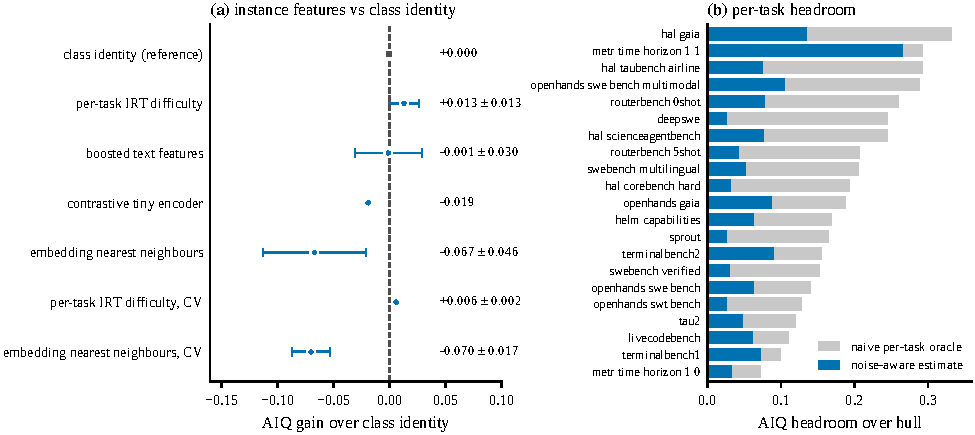
\includegraphics{fig-class-suff.pdf}
\caption{(a) AIQ gain over class identity for instance-level feature families (mean $\pm$ 95\% CI over seeds; S1: 21 matrices, three seeds; CV: DeepSWE five-fold, five seeds). (b) Per-matrix headroom over the single hull: the naive per-task oracle (grey) and a noise-aware estimate (blue; leave-one-run-out where repeats exist, a denoised IRT oracle otherwise).}
\label{fig:class}
\end{figure}

\subsection{Day-zero routing}
\label{sec:res-priors}

\Cref{fig:unseen} reports the paired gain over the class-mean router, with task-bootstrap confidence intervals. On a held-out model family (S5) the credibility prior adds $+0.153\ci{0.145}{0.163}$ AIQ; on a held-out benchmark family (S2), $+0.072\ci{0.062}{0.080}$; on held-out models with no anchors (S3, $K=0$), $+0.021\ci{0.010}{0.040}$. Removing the leaderboard aggregates leaves the S5 gain unchanged ($+0.158$ without, $+0.153$ with), so the metadata prior carries it.

\begin{figure}[tbp]
\centering
\begin{minipage}[t]{0.49\textwidth}\centering
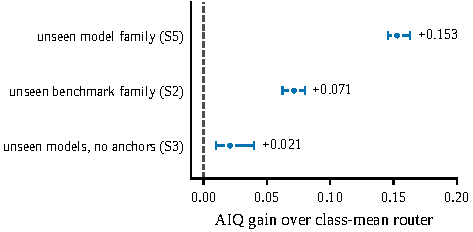
\includegraphics{fig-unseen.pdf}
\caption{Gain over the class-mean router on unseen model families (S5, 11 matrices), unseen benchmark families (S2, 21 matrices) and unseen models without anchors (S3, 21 matrices); paired task-bootstrap 95\% CIs.}
\label{fig:unseen}
\end{minipage}\hfill
\begin{minipage}[t]{0.49\textwidth}\centering
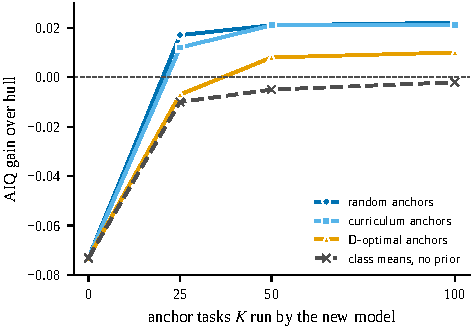
\includegraphics{fig-anchors.pdf}
\caption{Anchor curve on S3: AIQ gain over the single hull as a function of the number of anchor tasks a held-out model is run on, by anchor-selection rule (one seed, 21 matrices).}
\label{fig:anchors}
\end{minipage}
\end{figure}

\Cref{fig:anchors} is the anchor curve. With random anchors the gain over the single hull rises from $-0.073$ at $K=0$ to $+0.017$ at $K=25$ and $+0.022$ at $K=100$: the curve has saturated by 25 anchors. \Cref{prop:anchor} predicts saturation this fast only for the wide prior scale ($\varsigma_b=1.2$, $K_{1/2}\ge2.8$); with $\varsigma_b=0.3$ it would allow at most 36\% of the regret to be removed by $K=25$. The observed speed is therefore an empirical result, consistent with the wide-prior regime, and we did not record which scale validation selected on each matrix. Random anchors match or beat D-optimal ones at every $K$ ($+0.017$ vs $-0.007$ at $K=25$, $+0.022$ vs $+0.010$ at $K=100$), the failure mode of optimising information at a misspecified prior. A new model is routed from its metadata prior on day zero and reaches the saturated gain after 25 outcomes per class.

\subsection{Sequential Pareto search}
\label{sec:res-seq}

\Cref{fig:front} shows the DeepSWE quality--cost plane. The single-configuration hull tops out at 0.745 success for \$4.43 per task. A learned single-shot router tracks it, as \cref{thm:class} predicts for a benchmark whose tasks are close to exchangeable. The sequential policy moves the whole curve up and to the left: with a perfect verifier it reaches 0.94 success, and with an 80\%-accurate verifier it still lies above the hull over 95\% of the log-cost range, all except the cheapest end below \$0.10 per task.

\begin{figure}[tbp]
\centering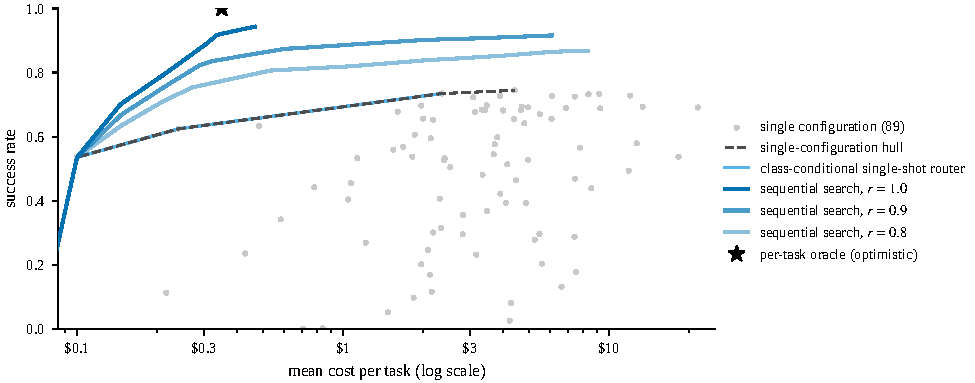
\includegraphics{fig-deepswe-front.pdf}
\caption{DeepSWE, 111 tasks $\times$ 89 configurations, 15 folds of held-out tasks. Grey points: single configurations; dashed: their hull; light blue: the class-conditional single-shot router; blue, darkest to lightest: the sequential Pandora-index policy at verifier accuracies $r=1.0,0.9,0.8$. The star is the per-task oracle, which exploits outcome noise and is not attainable.}
\label{fig:front}
\end{figure}

\begin{table}[tbp]
\centering\small
\begin{tabular}{lccccc}\toprule
 & $r=1$ & $r=0.9$ & $r=0.8$ & $r=0.7$ & $r=0.6$\\\midrule
\multicolumn{6}{l}{\emph{AIQ gain over the single-configuration hull (mean $\pm$ 95\% $t$-CI, 15 folds)}}\\
Pandora index & $+0.172\pm0.022$ & $+0.132\pm0.018$ & $+0.081\pm0.015$ & $+0.032\pm0.012$ & $-0.016\pm0.011$ \\
exact DP ($A{=}3$) & $+0.136\pm0.017$ & $+0.095\pm0.015$ & $+0.056\pm0.013$ & $+0.021\pm0.010$ & $-0.017\pm0.011$ \\
learned single-shot & $-0.030\pm0.013$ & $-0.030\pm0.013$ & $-0.030\pm0.013$ & $-0.030\pm0.013$ & $-0.030\pm0.013$ \\
\midrule
\multicolumn{6}{l}{\emph{cost per task to reach the best configuration's success (share of its cost)}}\\
Pandora index & \$0.18 (4\%) & \$0.21 (5\%) & \$0.26 (6\%) & \$0.59 (13\%) & \$3.75 (85\%) \\
exact DP ($A{=}3$) & \$0.17 (4\%) & \$0.20 (5\%) & \$0.34 (8\%) & \$0.94 (21\%) & \$4.62 (104\%) \\
\bottomrule\end{tabular}

\caption{Sequential policies on DeepSWE (111 tasks, 89 configurations, 5 folds $\times$ 3 repetitions, 12 real-trial draws per test task; every attempt consumes a different recorded trial). The best single configuration reaches 0.745 success at \$4.43 per task.}
\label{tab:seq}
\end{table}

\Cref{tab:seq} and \cref{fig:aiq} quantify it. The Pandora index gains $+0.172\pm0.022$ AIQ over the hull at $r=1$ and $+0.081\pm0.015$ at $r=0.8$, and it reaches the best configuration's success rate for \$0.18--\$0.26 per task, 4--6\% of that configuration's cost, for every $r\ge0.8$. The index beats the exact three-attempt dynamic program at every accuracy from 0.7 up (e.g.\ $+0.172$ vs $+0.136$ at $r=1$) because it may use up to six attempts. The gain is significantly positive for $r\ge0.7$ and negative at $r=0.6$, which is consistent with the sufficient threshold $\hat r^\ast=0.65$ of \cref{prop:est}; that threshold bounds the transition from above and does not predict the negative gain at 0.6.

\begin{figure}[tbp]
\centering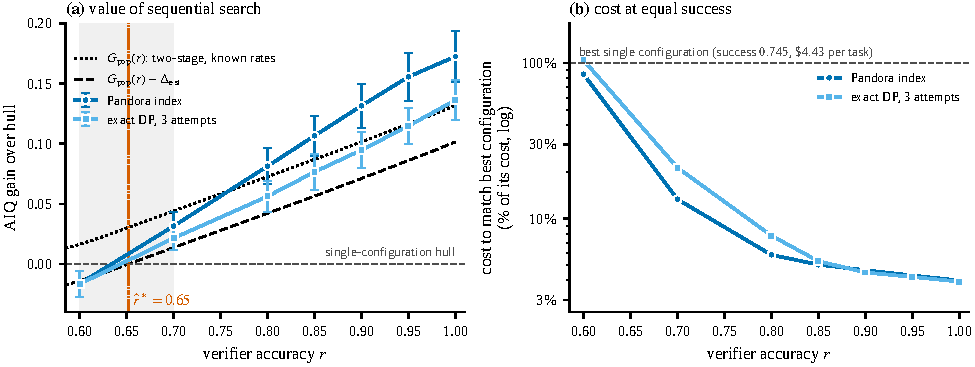
\includegraphics{fig-aiq-vs-r.pdf}
\caption{(a) AIQ gain over the single-configuration hull as a function of verifier accuracy (mean $\pm$ 95\% $t$-CI over 15 folds). Dotted: the population gain of static two-stage cascades, $G_{\rm pop}(r)$; dashed: $G_{\rm pop}(r)-\Delta_{\rm est}$; the dash-dotted line marks the predicted threshold $\hat r^\ast$ of \cref{prop:est}; the shaded band is the interval in which the observed gain changes sign. (b) Cost per task to reach the best single configuration's success rate, as a share of that configuration's cost.}
\label{fig:aiq}
\end{figure}

\paragraph{Correlated failures.} \Cref{prop:retry} makes the value of the second attempt depend on the covariance of failures, and DeepSWE allows a partial estimate of it. \Cref{tab:corr} lists every pair of hull configurations whose cheaper member succeeds on more than 10\% of tasks: failures are positively correlated in all six pairs (correlation between 0.17 and 0.40), and the covariance removes 0.04--0.08 of success probability from two attempts relative to independent attempts with the same success rates. In the fitted latent model the task difficulty has scale $\tau=1.64$, the base-model-by-task effect $\omega_{\rm base}=0.20$ and the configuration-by-task effect $\omega_m=1.50$ (logit units, means over 15 fits): the shared difficulty accounts for 54\% of the latent variance of a configuration's per-task logit, and the configuration-specific effect, which a retry of the same configuration repeats, for most of the rest. These estimates describe interactions between attempts of single-agent configurations, not between roles of a crew.

\begin{table}[tbp]
\centering\small
\begin{tabular}{rrrrrr}\toprule
$p_1$ & $p_2$ & $\mathrm{Corr}(y_1,y_2)$ & two attempts, independent & two attempts, observed & loss\\\midrule
0.536 & 0.626 & 0.29 & 0.827 & 0.756 & 0.070\\
0.536 & 0.735 & 0.17 & 0.877 & 0.839 & 0.038\\
0.536 & 0.741 & 0.22 & 0.880 & 0.831 & 0.049\\
0.626 & 0.735 & 0.22 & 0.901 & 0.853 & 0.048\\
0.626 & 0.741 & 0.28 & 0.903 & 0.845 & 0.059\\
0.735 & 0.741 & 0.40 & 0.931 & 0.854 & 0.077\\
\bottomrule\end{tabular}

\caption{Correlated failures between DeepSWE hull configurations (111 tasks; pairs whose cheaper member succeeds on at most 10\% of tasks omitted). The two attempts on a task are independent draws from each configuration's recorded trials, so the dependence is the one induced by per-task success rates that vary together across tasks. Corr: Pearson correlation of the two success indicators. Two attempts: probability that at least one succeeds, if attempts were independent and as observed; loss: their difference, which equals the covariance (\cref{prop:retry}).}
\label{tab:corr}
\end{table}

\subsection{Budget pacing}
\label{sec:res-pace}

\Cref{fig:pacing} runs the dual step \eqref{eq:pacing} on the exact dynamic-programming policy over five stream orders and six budgets per accuracy. For $r\le0.9$ the realised spend is within 3--13\% of the budget, and quality is within 0.011 of the best fixed $\lambda$ chosen in hindsight. With an exact verifier the policy concentrates spend on hard tasks (realised spend $1.39\times$ the budget, the heavy-tail term of \cref{prop:pace}) and still matches hindsight quality within 0.010.

\begin{figure}[tbp]
\centering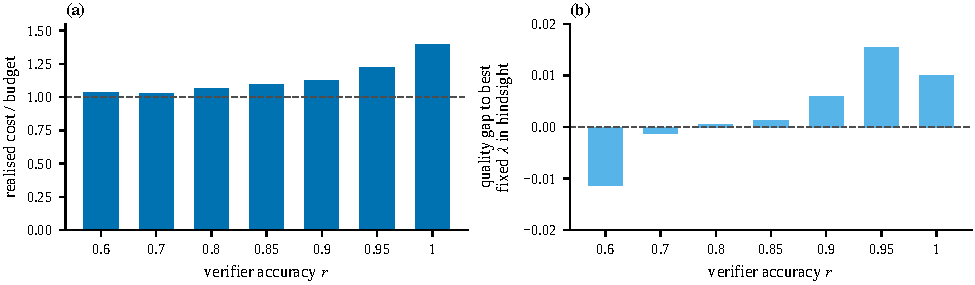
\includegraphics{fig-pacing.pdf}
\caption{Online dual pacing on DeepSWE (111-task streams, five orders $\times$ six budgets, $\vartheta=0.2$). (a) Realised mean cost over the budget. (b) Quality gap to the best fixed $\lambda$ in hindsight on the same stream.}
\label{fig:pacing}
\end{figure}

\subsection{The moving frontier}

\Cref{fig:frontier-time} replays the DeepSWE hull using only configurations whose models had been released by a given date. The price of 50\% success fell from \$4.64 to \$0.10 per task when a low-cost open-weight model arrived in late April; the price of 65\% fell from \$2.99 (July) to \$1.38 (August) to \$0.70 (September), and 70\% became reachable at \$12.49 in July and costs \$1.68 today. A router that re-reads the catalog and scores new models from metadata captures these drops on the day they happen; a static crew captures none of them.

\begin{figure}[tbp]
\centering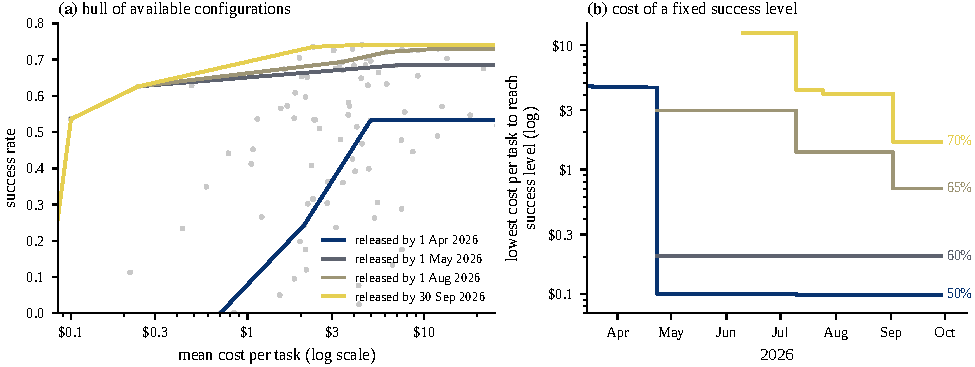
\includegraphics{fig-frontier-time.pdf}
\caption{(a) DeepSWE single-configuration hull restricted to models released by each date. (b) The lowest cost per task at which each success level is reachable, as a function of date.}
\label{fig:frontier-time}
\end{figure}

%======================================================================
\section{Real-world validation on GitHub issues}
\label{sec:trial}
%======================================================================

\paragraph{Design.}
We took 22 real, closed GitHub issues from 22 open-source Python repositories: 14 defect fixes and 8 open-ended feature or refactor tasks. Each issue was solved once by each crew configuration in the same harness, from the same base commit, with a wall-clock cap of 15 minutes per run. Every resulting change was scored by two independent reviewers, blind to configuration identity, on a 0--10 rubric with a mergeability verdict (\emph{yes}, \emph{with minor changes}, \emph{no}). A candidate is \emph{mergeable} if neither reviewer says \emph{no}, and \emph{good} if it is mergeable and its mean score is at least 7. The two reviewers agree closely: Spearman correlation 0.88 and ICC(2,1) $=0.90$ on the 0--10 scores over 103 doubly-reviewed candidates, and Cohen's $\kappa=0.83$ on the binary mergeability verdict (\cref{app:review}).

\paragraph{Configurations ($n=3$).}
The experiments instantiate the formalism with the three roles of CodeAF (worker, planner, checker). Two configurations are on the diagonal of the crew space (\cref{sec:diagonal}): the \emph{uniform low-cost crew} puts a low-cost open-weight model in every seat, and the \emph{uniform frontier crew} a frontier open-weight model in every seat. Three are off the diagonal. The \emph{low-cost-checker crew} keeps the low-cost worker and adds a second low-cost open-weight model as checker, and the \emph{strong-checker crew} keeps the low-cost worker and adds the frontier model as checker; both also place a mid-tier model in the planner seat, but no issue was decomposed into sub-tasks and the planner model was called only five times across all their runs. The agent also has an auxiliary probe role outside the three, which serves small calls; the strong-checker crew and the alternative worker use the second low-cost model there. The strong-checker crew therefore differs from the uniform low-cost crew in three seats (checker, planner, probe), of which the checker accounts for 71\% of the bill. We call it a checker upgrade below, but it is not a single-role change in the sense of \cref{def:leverage}, and the trial does not separate the checker's effect from the planner's and the probe's. The \emph{alternative low-cost worker} replaces the worker with a different low-cost model. \Cref{tab:models} lists the models and \cref{app:configs} the full seat mapping. The uniform low-cost, low-cost-checker and strong-checker crews were run on all 22 issues; the uniform frontier crew and the alternative worker were run on the 14 defect fixes only. On open-ended tasks, therefore, the only measured diagonal configuration is the uniform low-cost crew. The \emph{routed} policy is the router's class rule: the uniform low-cost crew on defect fixes and the strong-checker crew on open-ended tasks. Its outcome on each issue is the outcome of the configuration it selects, which was run on that issue.

\begin{table}[tbp]
\centering\small
\begin{tabularx}{\textwidth}{llrrX}\toprule
tier & model & \$/M in & \$/M out & roles in the trial\\\midrule
low-cost open-weight & \texttt{glm-5.3-flash} & 0.15 & 0.50 & worker (three crews), every role of the low-cost crew\\
low-cost open-weight & \texttt{deepseek-v4-flash} & 0.09 & 0.18 & checker (low-cost-checker crew), alternative worker\\
mid-tier open-weight & \texttt{glm-5.3} & 0.84 & 2.64 & planner (checker crews)\\
frontier open-weight & \texttt{kimi-k3} & 3.00 & 15.00 & checker (strong-checker crew), every role of the frontier crew\\
\bottomrule\end{tabularx}
\caption{Models in the real-issue trial with catalog prices per million tokens at the time of the study.}
\label{tab:models}
\end{table}

\paragraph{The routed policy matches the best fixed crew at 40\% lower cost.}
\Cref{tab:trial} gives the policy-level results. The routed policy scores $6.95\ci{6.30}{7.55}$ with 20 of 22 issues mergeable and 15 good, at \$0.057 per issue. The strong-checker crew on every issue scores the same, $6.95\ci{6.30}{7.57}$ (paired difference $0.00\ci{-0.75}{0.82}$), with 20 mergeable and 13 good, at \$0.095 per issue: routing cuts cost by 40\% at no measurable loss and two more good changes.

\begin{table}[tbp]
\centering\small
\begin{tabular}{lcccc}\toprule
policy & score [95\% CI] & mergeable & good ($\geq 7$) & cost / issue\\\midrule
routed (class-aware) & 6.95 [6.30, 7.55] & 20/22 & 15/22 & \$0.057 \\
strong-checker crew & 6.95 [6.30, 7.57] & 20/22 & 13/22 & \$0.095 \\
low-cost crew + low-cost checker & 6.05 [5.18, 6.84] & 17/22 & 10/22 & \$0.034 \\
uniform low-cost crew & 5.50 [4.64, 6.34] & 12/22 & 8/22 & \$0.032 \\
\bottomrule\end{tabular}

\caption{Policy-level results on 22 issues (14 defect fixes, 8 open-ended). Score: mean of two blind reviewers, 0--10, with a task-bootstrap 95\% CI. Mergeable: no reviewer rejects. Good: mergeable and score $\ge7$. Cost: mean provider bill per issue, all seats.}
\label{tab:trial}
\end{table}

\paragraph{Crews against single-model policies.}
\Cref{fig:crew-frontier} places every configuration in the cost--quality plane and separates the diagonal from the crew frontier. Across all 22 issues the best measured diagonal policy is the uniform low-cost crew (the uniform frontier crew was not run on open-ended tasks); the class-aware crew improves on it by $+1.45\ci{0.64}{2.39}$ review points and raises mergeable changes from 12 to 20, for \$0.025 more per issue (\cref{fig:crew-frontier}c). The two classes contribute differently.
\begin{itemize}
\item \emph{Open-ended tasks: the best measured crew is off the diagonal.} The strong-checker crew adds $+4.00\ci{3.19}{4.94}$ points over the uniform low-cost crew and turns 0 of 8 mergeable changes into 8 of 8, at 2.4 times the cost; the crew frontier rises well above the only measured diagonal point (\cref{fig:crew-frontier}b). This establishes an off-diagonal optimum only among the measured crews. The worker's leverage was not measured on these tasks, and a uniform frontier crew was not run, so whether the optimum over all crews is off the diagonal is not identified.
\item \emph{Defect fixes: the best measured crew is on the diagonal.} Both uniform crews were run, and the diagonal frontier coincides with the crew frontier (\cref{fig:crew-frontier}a). No off-diagonal crew scores higher than the uniform frontier crew: the strong-checker crew differs by $-0.29\ci{-1.18}{0.50}$ points at 4.2 times lower cost, the low-cost-checker crew by $-0.61\ci{-1.50}{0.36}$ and the alternative worker by $-0.86\ci{-1.75}{0.14}$. The uniform low-cost crew differs by $-0.29\ci{-1.00}{0.46}$ at 15.4 times lower cost. On the point estimates the $\lambda$-optimal crew among the measured ones is uniform at every $\lambda$: the frontier crew below $\lambda\approx0.9$ review points per dollar and the low-cost crew above it.
\end{itemize}
Among the measured crews, the best crew is therefore heterogeneous on one class and uniform on the other (\cref{tab:choice}). A single-model router can express the defect-fix choice but not the open-ended one, and a fixed crew can express only one of the two; the class-aware crew expresses both.

\begin{figure}[tbp]
\centering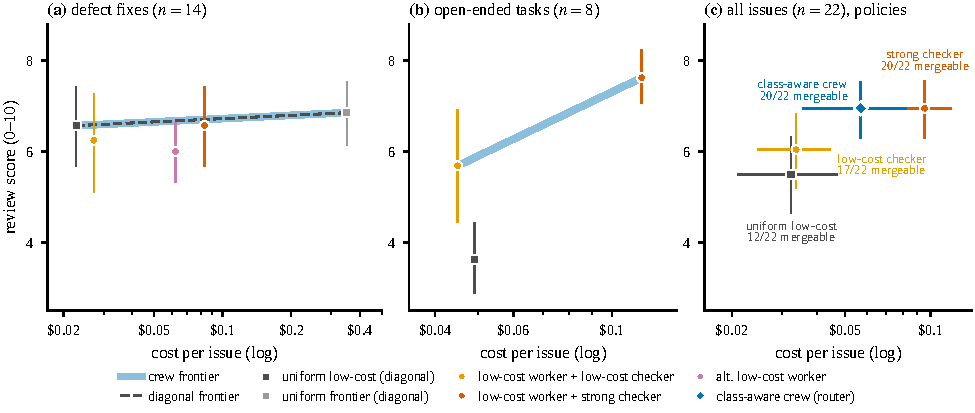
\includegraphics{fig-crew-frontier.pdf}
\caption{Crew frontier against the diagonal on real GitHub issues. Squares: diagonal (uniform) crews; circles: off-diagonal crews; bars: task-bootstrap 95\% CIs. Blue band: crew frontier (upper hull of all configurations); dashed: diagonal frontier (upper hull of the uniform crews). (a) Defect fixes: both uniform crews were run, and the frontiers coincide; the best measured crew is uniform. (b) Open-ended tasks: only the uniform low-cost crew was run on the diagonal; the frontier of the measured crews is attained off the diagonal by the strong-checker crew. (c) Policies on all 22 issues, with cost CIs on both axes and the number of mergeable changes.}
\label{fig:crew-frontier}
\end{figure}

\paragraph{Role attribution: the checker effect is specific to open-ended tasks.}
\Cref{fig:seat} and \cref{fig:trial} give paired differences against the uniform low-cost crew; as noted above, the checker upgrade also changes the planner and probe seats. On open-ended tasks, the strong checker adds $+4.00\ci{3.19}{4.94}$ points; even a low-cost checker adds $+2.06\ci{0.50}{3.63}$, and the strong checker beats it by $+1.94\ci{0.63}{3.25}$. The effect replicates across the three separately collected batches of open-ended issues ($+3.7$, $+3.8$, $+4.8$; $n=3,3,2$). On defect fixes, the strong checker adds $0.00\ci{-1.25}{1.14}$, and the frontier model in every seat adds $+0.29\ci{-0.46}{1.00}$ at 15 times the cost. This is the pattern \cref{ex:verify} predicts: the low-cost worker already produces a mergeable fix for 12 of 14 defects, so there is little for a checker to catch, while its first attempt at open-ended work is never mergeable. The strong checker is 71\% of the strong-checker crew's bill, which is why spending it only where it pays cuts the policy's cost by 40\%.

\begin{figure}[tbp]
\centering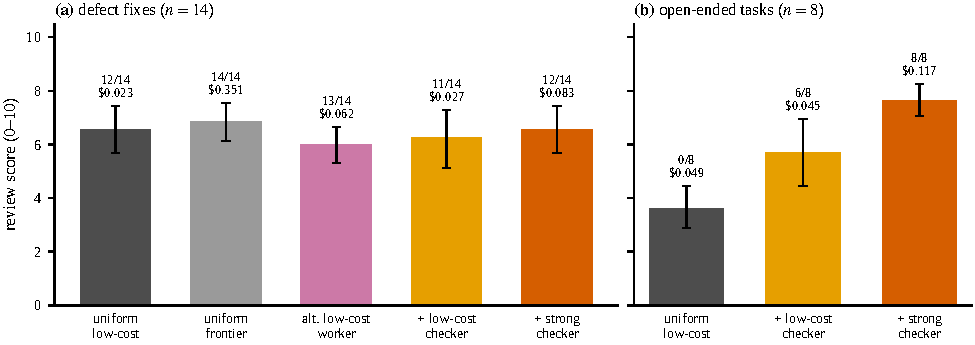
\includegraphics{fig-trial-class.pdf}
\caption{Mean review score by issue class and configuration (task-bootstrap 95\% CIs). Above each bar: mergeable issues and mean cost per issue. The uniform frontier crew and the alternative low-cost worker were run on defect fixes only.}
\label{fig:trial}
\end{figure}

\paragraph{What the trial identifies about interactions.} The trial was not designed as a factorial over roles. The frontier model occupies the checker seat with a low-cost worker (strong-checker crew, which also changes the planner and probe) and every seat together (uniform frontier crew, defect fixes only); it never occupies the worker seat alone. Because a frontier worker with a low-cost checker was never run, the worker--checker interaction $I_{st}$ of \eqref{eq:interact} is not identified, and we report no interaction matrix. Two contrasts are identified. On defect fixes, with the frontier checker in place, upgrading the worker and planner to the frontier model changes the score by $+0.29\ci{-0.50}{1.18}$ at 4.2 times the cost, and upgrading the checker of the low-cost crew changes it by $0.00\ci{-1.25}{1.14}$. Across classes, the checker upgrade gains $+4.00\ci{2.54}{5.56}$ points more on open-ended tasks than on defect fixes (independent task bootstrap per class). This is a class-by-role interaction, not a role-by-role one, but it has the sign and the ordering that \cref{ex:verify} predicts from the low-cost worker's error rate: the uniform low-cost crew leaves 8 of 8 open-ended changes and 2 of 14 defect fixes unmergeable, so the checker's leverage should be up to seven times larger on open-ended work.

\Cref{tab:leverage} expresses the same contrasts as the role gains and leverage ratios of \cref{def:leverage}. Upgrading the checker on open-ended tasks has a leverage ratio of about 59 review points per dollar per issue; upgrading every role on defect fixes has a ratio of 0.9. By \cref{prop:rule}, among the measured configurations the $\lambda$-optimal crew upgrades the checker on open-ended tasks and keeps the uniform low-cost crew on defect fixes for any $\lambda$ between these values, and among the measured open-ended crews the optimum is off the diagonal. This is the assignment in \cref{tab:choice}. The data do not support role-level conclusions beyond this. An all-roles leverage below $\lambda$ does not imply that every single role's leverage is below $\lambda$, since under additivity the role gains add and one role could exceed $\lambda$ while another is negative. The worker's leverage on open-ended tasks was not measured.

\begin{table}[tbp]
\centering\small
\begin{tabular}{lllrl}\toprule
class & upgrade & $\Delta_s$ & $\Delta c_s$ (\$) & $\Lambda_s$ (points/\$)\\\midrule
open-ended & checker: low-cost $\to$ frontier & +4.00 [+3.19, +4.94] & +0.068 & 59.2\\
open-ended & checker: low-cost $\to$ second low-cost & +2.06 [+0.50, +3.62] & $-$0.004 & dominant ($\Delta c_s\le0$)\\
defect fix & checker: low-cost $\to$ frontier & +0.00 [$-$1.25, +1.14] & +0.060 & 0.0\\
defect fix & checker: low-cost $\to$ second low-cost & $-$0.32 [$-$1.36, +0.75] & +0.004 & $-$71.8\\
defect fix & all roles: low-cost $\to$ frontier & +0.29 [$-$0.46, +1.00] & +0.328 & 0.9\\
\bottomrule\end{tabular}

\caption{Role gains $\Delta_s$ (paired, review points on 0--10, task-bootstrap 95\% CI), marginal cost $\Delta c_s$ per issue and leverage ratio $\Lambda_s$ (points per dollar), relative to the uniform low-cost crew ($n=3$). The two checker rows compare crews that also differ in the planner and probe seats (\cref{sec:trial}), so they are multi-seat contrasts dominated by the checker; a negative $\Lambda_s$ reflects a point estimate below zero, not a violation of \cref{ass:mono}.}
\label{tab:leverage}
\end{table}

\begin{table}[tbp]
\centering\small
\begin{tabular}{llllcccc}\toprule
class & worker & planner & checker & on diagonal & score & mergeable & cost / issue\\\midrule
defect fix & low-cost & low-cost & low-cost & yes & 6.57 & 12/14 & \$0.023\\
open-ended & low-cost & mid-tier & frontier & no & 7.62 & 8/8 & \$0.117\\
\bottomrule\end{tabular}
\caption{Class-conditional assignment of the routed policy for the $n=3$ roles of CodeAF (models in \cref{tab:models}), with its results per class. Among the measured configurations, the best crew is uniform on defect fixes and heterogeneous on open-ended tasks.}
\label{tab:choice}
\end{table}

\begin{figure}[tbp]
\centering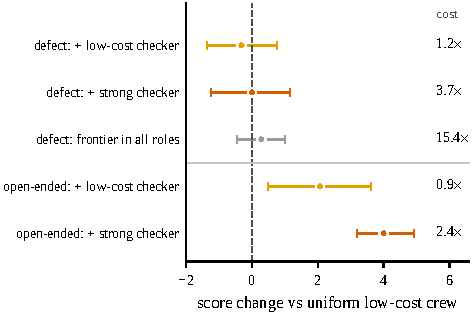
\includegraphics{fig-seat.pdf}
\caption{Role attribution ($n=3$): paired score change relative to the uniform low-cost crew on the same issues, with task-bootstrap 95\% CIs and the cost multiple of each change.}
\label{fig:seat}
\end{figure}

%======================================================================
\section{System and deployment}
\label{sec:system}
%======================================================================

The method is implemented as the model-routing component of the CodeAF coding agent, as a table embedded in the agent binary. A routing decision is a local computation with no network call and no language-model call. \Cref{tab:size} gives the measured footprint.

\begin{table}[tbp]
\centering\small
\begin{tabular}{lrrl}\toprule
predictor & size (MB) & latency (ms) & runs\\\midrule
Pareto Crewing router (classifier + priors) & 0.1--1.1 & 0.6--0.7 & in the agent binary, one CPU core\\
class-mean table & 0.2 & 0.8 & in process\\
full hierarchical IRT stack & 8.2 & 815 & offline fitting\\
embedding nearest neighbours & 240--384 & 220--455 & dedicated service\\
\bottomrule\end{tabular}
\caption{Inference artifact size and single-task CPU latency (median, predictions for all candidates) across evaluation splits.}
\label{tab:size}
\end{table}

\paragraph{Size.} The routing artifact is the classifier weights (8-bit, at most 2{,}000 per class), the per-(class, role, model) prior table with its credibility counts, and the metadata regression $W$: 0.1--1.1\,MB depending on the number of units, compared with 240--384\,MB for the embedding-based router in \cref{tab:size}.

\paragraph{Latency and throughput.} Predictions for all candidates take 0.6--0.7\,ms per task on one CPU core, over 1{,}400 routing decisions per second per core. The per-seat argmax of \cref{prop:seat} adds a linear scan over the (model, route) pairs. For a task that runs for one minute, routing accounts for about $10^{-5}$ of wall-clock time.

\paragraph{Coverage.} Every model reachable through a pay-per-token API, a subscription or a local runtime is a candidate, priced at its route-aware marginal cost \eqref{eq:cost}. A newly released model is routed through its metadata prior before any of its outcomes are observed (\cref{sec:res-priors}); its own outcomes then update the prior through the credibility blend (\cref{prop:cred}).

%======================================================================
\section{Related work}
%======================================================================

\paragraph{Call-level routing and cascades.}
RouteLLM learns a binary strong/weak router from preference data \cite{ong2024routellm}; Hybrid LLM routes on predicted quality gaps \cite{ding2024hybrid}; RouterBench \cite{hu2024routerbench}, SPROUT/CARROT \cite{somerstep2025carrot} and EmbedLLM \cite{zhuang2025embedllm} provide corpora and learned model embeddings. FrugalGPT \cite{chen2023frugalgpt}, AutoMix \cite{madaan2024automix} and mixture-of-thought cascades \cite{yue2024cascades} escalate from cheap to strong models using a scorer or self-verification. All of these are call-level routers in the sense of \cref{def:levels}: they choose one model, or one sequence of models, per call and evaluate the choice by that call's own outcome. Applied to an agent with several roles, they either select among uniform crews, the diagonal of the crew space, or optimise a role-additive surrogate that cannot represent interactions between roles (\cref{prop:call}). Pareto crewing routes at the task level: it assigns a model to each role, scores the crew by the whole trajectory's quality and cost, attains a frontier at least as good as any diagonal router over the same candidates (\cref{prop:dominance}), and reduces to single-model routing when $n=1$. Cascades correspond to our sequential layer, for which we give the verifier accuracy at which they pay (\cref{thm:rstar}) and the loss from correlated failures (\cref{prop:retry}).

\paragraph{Item response theory for model evaluation.}
IRT has been used to compress benchmarks and to predict model performance from few items \cite{polo2024tinybenchmarks}. We use a three-parameter model with a hierarchical, metadata-driven prior on abilities and leaderboard aggregates as moment constraints \cite{quadrianto2009,hansen1982gmm}, fitted by marginal likelihood with quadrature \cite{bock1981}, and read the posterior through credibility theory \cite{buhlmann1967}.

\paragraph{Search and budgets.}
Our sequential layer is Weitzman's Pandora's box \cite{weitzman1979} with a noisy inspection and correlated boxes; nonobligatory inspection \cite{doval2018} and the descending-price view \cite{kleinberg2016} are related extensions. Budget pacing follows the online-allocation literature on bandits with knapsacks \cite{badanidiyuru2018,agrawal2014} and dual mirror descent \cite{balseiro2020}. Seat-level structure relates to combinatorial semi-bandits \cite{chen2013cmab}.

\paragraph{Evaluation with model judges.}
Our real-issue endpoint uses model-based reviewers, whose agreement with human preferences has been studied extensively \cite{zheng2023judge}; we report inter-reviewer reliability \cite{shrout1979,cohen1960} and bootstrap intervals \cite{efron1993}.

%======================================================================
\section{Conclusion}
%======================================================================

We formulated task-level multi-model routing: the joint assignment of models to the $n$ roles of an agent crew, per task, scored by the quality and cost of the whole trajectory. Call-level routing is its restriction to role-additive surrogates, and single-model routing its further restriction to the diagonal of the crew space. The crew frontier weakly dominates the diagonal frontier for any quality function, number of roles and number of objectives; it is strictly better at some budgets when the roles' leverage ratios straddle a non-negative price of quality, and, for two roles, when one role compensates for the other's errors, even if one model has the highest additive score in both roles. Role interactions and correlated failures are parameterised in a latent space conditioned on the task class, which approximate class sufficiency justifies: instance-level information adds at most about 0.01 AIQ. The experiments instantiate $n=3$ roles and two objectives. On real GitHub issues the best measured crew is heterogeneous and class-dependent: on open-ended tasks it upgrades a subset of the low-cost crew's roles and raises mergeable changes from 0/8 to 8/8 over the uniform low-cost crew, while on defect fixes it is a uniform crew, and the uniformly low-cost crew matches the uniformly frontier crew at $15.4\times$ lower cost. The gain from that role differs between the two classes in the direction that the compensation result predicts from the error rate of the other roles; the trial does not identify single-role effects or the pairwise interaction between roles. The class-aware crew matches the best fixed crew at $1.68\times$ lower cost and improves on the best measured single-model policy by $+1.45$ points. On DeepSWE, failures of different configurations are positively correlated, which lowers the value of repeated attempts, and sequential search still reaches the best configuration's success rate at 17--25$\times$ lower cost given a verifier of accuracy at least 0.8. Because the frontier moved 46-fold in one month on the benchmark we studied, continuous re-optimisation of the crew is both necessary and inexpensive.

\bibliographystyle{plainnat}
\bibliography{refs}

%======================================================================
\appendix
\section{Notation}
\label{app:notation}
\Cref{tab:notation} lists the symbols used in more than one section. A few letters keep a second, local meaning inside a single paragraph or proof; these are listed in the last block of the table.

{\small
\begin{longtable}{@{}p{0.27\textwidth}p{0.69\textwidth}@{}}
\caption{Notation.}\label{tab:notation}\\
\toprule symbol & meaning\\\midrule\endfirsthead
\toprule symbol & meaning\\\midrule\endhead
\bottomrule\endfoot
\multicolumn{2}{@{}l}{\emph{Crews, costs and frontiers}}\\
$n$, $\seats$, $s,t$ & number of roles, the set of roles, role indices\\
$\mods$, $\mods_s$, $\mods_\cap$, $m$ & configurations ((model, route) pairs), those admissible in role $s$, those admissible in every role, a configuration\\
$\mu$, $\nu$ & the model and the route of a configuration\\
$\crew=(m_1,\dots,m_n)$, $\mathcal D$ & a crew; the diagonal (uniform crews over $\mods_\cap$)\\
$c\in\cls$, $x_t$, $\psi(c\mid x)$ & task class, task description, calibrated class posterior\\
$c_s(m;c)$, $C(\crew;c)$ & expected cost of role $s$ with configuration $m$; expected crew cost (\$ per task)\\
$C_t$, $C_{tm}$, $C_k$ & realised cost of task $t$, of configuration $m$ on task $t$, of call $k$\\
$Q(\crew;c)$, $y_{tm}$ & expected quality (success probability); success indicator of $m$ on task $t$\\
$\pi$ & a routing policy (a distribution over crews, per class or per description)\\
$B$, $B_{\min}$, $F$, $F_{\rm crew}$, $F_{\rm diag}$ & budget (\$ per task), cheapest feasible budget, frontier over all crews and over $\mathcal D$\\
$\lambda$, $L_\lambda=Q-\lambda C$ & price of quality (quality per \$); Lagrangian\\
$B_{\rm lo},B_{\rm hi}$, $u=\log B$ & AIQ budget range and log budget\\
$(u_0,F_0)$, $(u_1,F_1)$, $\bar d$, $u^\star$, $\lambda_{\rm knee}$ & knee endpoints, chord slope, knee, knee multiplier\\
$\alpha$, $\beta_0$ & price rescaling and quality shift in \cref{prop:knee}\\
\multicolumn{2}{@{}l}{\emph{Interactions and leverage}}\\
$\crew^0$, $q_0$, $q_s$, $I_{st}$, $R$ & reference crew, baseline, main effect of role $s$, pairwise interaction, remainder \eqref{eq:interact}\\
$Q_{\rm add}$, $Q_{\rm int}$, $\eta$ & additive and interaction parts of $Q$; range of the interaction part\\
$\delta_s$, $g_s(m)$ & additive role effect ($=q_s$ under \cref{ass:add}); role utility $\delta_s(m;c)-\lambda c_s(m;c)$\\
$\Delta_s$, $\Delta c_s$, $\Lambda_s$ & role gain, marginal cost, leverage ratio $\Delta_s/\Delta c_s$ (\cref{def:leverage})\\
$\Lambda_{t\mid x}$ & leverage of role $t$ from $a$ to $b$ when role $s$ holds $x$ (\cref{prop:complement})\\
$G_n(\lambda)$ & Lagrangian gap between crews and diagonal with $n$ roles (\cref{prop:gap})\\
$d$, $\mathbf o$, $w$ & number of objectives, objective vector, positive weights\\
$A$, $A_x$, $\beta_j$, $\varphi$, $J$ & acceptance probability of the producing roles; sensitivity of reviewer $j$; repair probability; number of reviewers (\cref{ex:verify})\\
\multicolumn{2}{@{}l}{\emph{Priors}}\\
$u$ (Level 1--2), $b$ & a unit (benchmark or subset), a benchmark\\
$\zeta_{um}$, $\theta_m$, $S_{bm}$ & Level-1 logit, latent ability, published score\\
$\ell_{um}$, $\ell^0_{um}$, $\hat\ell$, $\tilde\ell$ & Level-2 intercept, its prior mean, posterior mean, maximum-likelihood value\\
$z_t$, $\tau_u$, $\kappa_m$, $g_u$ & task difficulty, its spread, discrimination, guessing floor\\
$\varsigma_b$, $\varsigma$ & prior scale of $\ell$\\
$\bar I$, $Z$, $n_0$ & mean observed information per task, credibility weight, credibility constant\\
$K$, $K_{1/2}$, $v_K$, $\mathrm{Reg}$, $H$ & anchors, half-saturation anchor count, posterior variance, regret, its curvature\\
$\varepsilon$ & exchangeability tolerance in \cref{thm:class}\\
\multicolumn{2}{@{}l}{\emph{Sequential search and pacing}}\\
$r$, $v$ & verifier accuracy $\Pr(v=y)$, verifier signal\\
$p$, $P_+$, $x_\pm$, $\sigma$ & prior correctness, pass probability, posterior correctness after pass/fail, reservation index\\
$\rho=C_1/C_2$, $p_{10},p_{01}$, $\chi$, $D$, $r^\ast$ & cost ratio, discordance probabilities, and the quantities of \cref{thm:rstar}\\
$G(r)$, $G_{\rm pop}(r)$, $\Gamma(r)$ & advantage over the chord; population and learned AIQ gain of two-stage search\\
$\Delta_{\rm est}$, $\Delta_{\rm adapt}$, $\hat r^\ast$ & estimation loss, residual value of adaptivity, sufficient accuracy threshold\\
$e_{tm}$, $u_{t,{\rm base}}$, $\omega_m$, $\omega_{\rm base}$ & task$\times$configuration and task$\times$base-model effects and their spreads\\
$\vartheta$, $\bar\lambda$, $T$ & pacing step, bound on $\lambda_t$, number of tasks\\
\multicolumn{2}{@{}l}{\emph{Local meanings}}\\
$\alpha_u,\beta_u,\gamma$, $w_{um}$, $\varepsilon_m$ & Level-1 loadings, offsets, effort shifts, cell weights, configuration noise \eqref{eq:level1}\\
$G$, $(z_g,\omega_g)$ & quadrature nodes and weights \eqref{eq:ghq}\\
$G_c$ & distribution of task difficulty within class $c$\\
$\phi$, $\phi_0$ & remaining quota fraction of a subscription route and its threshold\\
$e(r)$ & escalation probability in \cref{thm:rstar}\\
$k$, $r_k$ & call index and per-call reward (\cref{def:levels})\\
\end{longtable}}

\section{Proofs}
\label{app:proofs}
%======================================================================

\begin{proof}[Proof of \cref{prop:duality}]
For each class $c$ let $\Delta_c$ be the simplex of distributions over its admissible crews. Problem \eqref{eq:primal} maximises the linear function $\sum_c w_c\sum_\crew\pi_c(\crew)Q(\crew;c)$ over $\prod_c\Delta_c$ subject to one linear inequality, where $w_c$ is the class frequency. The feasible set is a non-empty polytope whenever $B\ge B_{\min}$, so strong duality holds \cite{boyd2004}: $F(B)=\min_{\lambda\ge0}\{\lambda B+\max_{\pi}\sum_c w_c\sum_\crew\pi_c(\crew)[Q-\lambda C]\}$, and the inner maximum is attained at a vertex, i.e.\ a deterministic $\crew_\lambda$ per class. $F$ is the value function of a parametric linear program in the right-hand side, hence concave and piecewise linear; it is non-decreasing because the constraint relaxes with $B$. A vertex of $F$ is where the minimising $\lambda$ changes, and it is attained by the argmax policy at any $\lambda$ in the open interval of multipliers supporting it; between two vertices the optimum mixes the two adjacent argmax policies with the weight that meets the budget with equality.
\end{proof}

\begin{proof}[Proof of \cref{prop:dominance}]
(i) $\mathcal D\subseteq\mods_1\times\dots\times\mods_n$, so a maximum over the larger set is at least the maximum over the smaller. Any randomised policy over $\mathcal D$ is a randomised policy over all crews with the same expected quality and cost, so the feasible set of \eqref{eq:primal} restricted to $\mathcal D$ is contained in the unrestricted one, and $F_{\rm crew}(B)\ge F_{\rm diag}(B)$.

(ii) Under \cref{ass:add}, $\max_\crew L_\lambda=q_0+\sum_s\max_{m\in\mods_s}g_s(m)$ by \cref{prop:seat}, and $\max_{\crew\in\mathcal D}L_\lambda=q_0+\max_{m\in\mods_\cap}\sum_sg_s(m)$. For every $m\in\mods_\cap$, $\sum_sg_s(m)\le\sum_s\max_{\mods_s} g_s$, with equality if and only if $m$ maximises every $g_s$ over $\mods_s$; since the sets are finite, the maxima are attained and the inequality between them is strict if and only if no such $m$ exists. With $\mods_s=\{a,b\}$, $g_s(b)-g_s(a)=(c_s(b)-c_s(a))(\Lambda_s-\lambda)$, which is positive for a role attaining $\max_s\Lambda_s>\lambda$ and negative for a role attaining $\min_s\Lambda_s<\lambda$. The first role's unique maximiser is $b$ and the second's is $a$, so there is no common maximiser; the optimal crew assigns $b$ to the first and $a$ to the second and is off the diagonal, and its value exceeds $\max\{L_\lambda(a,\dots,a),L_\lambda(b,\dots,b)\}$, the diagonal optimum.

(iii) Let $\mathcal H$ be the set of (expected cost, expected quality) pairs attained by randomised policies over a crew set, and set $F(B)=-\infty$ where no policy is feasible. For $\lambda\ge0$, $h(\lambda)=\max_{(C,Q)\in\mathcal H}(Q-\lambda C)=\sup_B\,[F(B)-\lambda B]$: for $(C,Q)\in\mathcal H$, $F(C)-\lambda C\ge Q-\lambda C$; conversely $F(B)$ is attained by some $(C',Q')\in\mathcal H$ with $C'\le B$, and $Q'-\lambda C'\ge F(B)-\lambda B$. A linear function on the polytope $\mathcal H$ is maximised at a vertex, a deterministic crew, so $h(\lambda)=\max L_\lambda$ over that crew set. If $F_{\rm crew}=F_{\rm diag}$ at every $B$ (with the $-\infty$ convention), the two support functions coincide. Hence a strict inequality $\max_\crew L_\lambda>\max_{\crew\in\mathcal D}L_\lambda$ at some $\lambda$ implies $F_{\rm crew}(B)\ne F_{\rm diag}(B)$ for some $B$, and by (i) $F_{\rm crew}(B)>F_{\rm diag}(B)$. If $\mathcal D$ contains a minimum-cost crew, both frontiers are finite exactly for $B\ge B_{\min}$ and equal to $-\infty$ below, so the budget at which they differ satisfies $B\ge B_{\min}$ and $F_{\rm diag}(B)$ is finite. Without that condition the difference may lie only at budgets below the cheapest diagonal crew, where $F_{\rm diag}=-\infty$. For a distribution over classes, the population problem decomposes by class under a common $\lambda$ (\cref{prop:duality}), so the population support function is the expectation of the class support functions; a strict inequality on a class of positive probability is strict in expectation, and the same argument applies.
\end{proof}

\begin{proof}[Proof of \cref{prop:gap}]
Let $g_1,\dots,g_{n+1}$ be the role utilities at $\lambda$ over the common candidate set $\mods$, and $S_n(m)=\sum_{s\le n}g_s(m)$. By (ii) above, $G_n=\sum_{s\le n}\max g_s-\max_m S_n(m)$. Then
\[
G_{n+1}-G_n=\max_m g_{n+1}(m)-\Big(\max_m\big[S_n(m)+g_{n+1}(m)\big]-\max_m S_n(m)\Big)\ge0,
\]
since $\max_m[S_n(m)+g_{n+1}(m)]\le\max_mS_n(m)+\max_mg_{n+1}(m)$. The constant $q_0$ appears in both maxima and cancels.
\end{proof}

\begin{proof}[Proof of \cref{prop:call}]
(i) Each call's objective depends only on its role and model, so the router's choice for the calls of role $s$ maximises $\bar r_s(m;c)-\lambda c_s(m;c)$ over $m\in\mods_s$, independently of the other roles; the resulting crew is $\hat\crew$. It is one of the admissible crews over which the task-level maximum is taken. (ii) $\hat\crew$ is a function of $\bar r_s$ and $c_s$ only, which do not involve $I_{st}$ or $R$. (iii) With $\bar r_s=q_s$, $\hat\crew$ maximises the additive part $Q_{\rm add}=q_0+\sum_sq_s$ of \eqref{eq:interact} minus $\lambda C$, and \cref{prop:interact} with $Q_{\rm int}=\sum_{s<t}I_{st}+R$ gives the bound; under \cref{ass:add} the bound is zero.
\end{proof}

\begin{proof}[Proof of \cref{prop:complement}]
(i) $L_\lambda(a,b)-L_\lambda(a,a)=Q(a,b)-Q(a,a)-\lambda\Delta c_t=\Delta c_t(\Lambda_{t\mid a}-\lambda)>0$ and $L_\lambda(a,b)-L_\lambda(b,b)=-(Q(b,b)-Q(a,b))+\lambda\Delta c_s=\Delta c_s(\lambda-\Lambda_{s\mid b})>0$. Both pair-uniform crews are therefore strictly worse than $(a,b)$, and the maximiser over the four crews is $(a,b)$ or $(b,a)$, both off the diagonal. (ii) The surrogate's main effects against $(b,b)$ are the losses $Q(b,b)-Q(a,b)=\Delta c_s\Lambda_{s\mid b}$ for moving role $s$ to $a$ and $Q(b,b)-Q(b,a)=\Delta c_t\Lambda_{t\mid b}$ for role $t$; by \cref{prop:rule} applied to the additive surrogate it upgrades role $s$ if and only if $\Lambda_{s\mid b}>\lambda$ and role $t$ if and only if $\Lambda_{t\mid b}>\lambda$, so above both ratios it selects $(a,a)$. On the stated interval the hypothesis of (i) holds. Compensation gives $\Lambda_{t\mid a}>\Lambda_{t\mid b}$, so the interval $(\max\{\Lambda_{s\mid b},\Lambda_{t\mid b}\},\Lambda_{t\mid a})$ is non-empty exactly when also $\Lambda_{s\mid b}<\Lambda_{t\mid a}$. The contrast identity follows by adding and subtracting $Q(b,a)$: $Q(a,b)-Q(a,a)-(Q(b,b)-Q(b,a))=\Delta c_t(\Lambda_{t\mid a}-\Lambda_{t\mid b})$, and symmetrically with the roles exchanged.
\end{proof}

\begin{proof}[Proof of \cref{prop:retry}]
$\Pr(y_1=0,y_2=0)=\E[(1-y_1)(1-y_2)]=(1-p_1)(1-p_2)+\mathrm{Cov}(y_1,y_2)$, and the probability of at least one success is its complement. With an exact verifier the second attempt is run only after a failure, so its value is $\Pr(y_1=0,y_2=1)=p_2-\Pr(y_1=1,y_2=1)=(1-p_1)p_2-\mathrm{Cov}(y_1,y_2)$.
\end{proof}

\paragraph{Multiple objectives.} Part (i) for $d$ objectives uses only $\mathcal D\subseteq\prod_s\mods_s$: every expected objective vector of a randomised diagonal policy is that of a randomised crew policy. With $w\in\R^d_{>0}$, a maximiser of $\langle w,\mathbf o\rangle$ is Pareto-optimal, since a dominating crew would have a strictly larger weighted sum; with $w\ge0$ only weak Pareto optimality follows. By Carath\'eodory's theorem a point on a face of the $d$-dimensional attainable set is a mixture of at most $d$ vertices. The characterisation in (ii) repeats the proof above with $g_s=\langle w,\mathbf o_s\rangle$, which is separable over roles when every objective is additive over roles. For (iii), if the support functions of the crew and diagonal attainable sets differ in direction $w$, the crew set contains a point $\mathbf o^\ast$ with $\langle w,\mathbf o^\ast\rangle$ larger than every diagonal point, and no diagonal point weakly dominates $\mathbf o^\ast$, since weak dominance with $w>0$ would give a weighted sum at least as large.

\begin{proof}[Proof of \cref{prop:knee}]
Under $B\mapsto\alpha B$, $u\mapsto u+\log\alpha$ for every point and both endpoints, so $u-u_0$ and $u_1-u_0$ are unchanged and the bracket in \eqref{eq:knee} is unchanged at each point; the tie-break is preserved. A shift $F\mapsto F+\beta_0$ cancels in $F-F_0$ and in $F_1-F_0$. For the slope condition, write $\mathcal K(u)=F(e^u)-F_0-\bar d(u-u_0)$. Since $F$ is concave in $B$, it has one-sided derivatives $F'_\pm$, and $\partial_u^\pm F(e^u)=e^uF'_\pm(e^u)$. At an interior maximiser of $\mathcal K$ its left derivative is $\ge0$ and its right derivative is $\le0$, so $\partial_u^+F(e^{u^\star})\le\bar d\le\partial_u^-F(e^{u^\star})$. Dividing by $B^\star=e^{u^\star}$ gives $F'_+(B^\star)\le\lambda_{\rm knee}\le F'_-(B^\star)$, so $\lambda_{\rm knee}$ is a supergradient of the concave $F$ at $B^\star$, i.e.\ a supporting multiplier. $\mathcal K$ need not be concave in $u$ (a linear piece of $F$ in $B$ is convex in $u$), so the maximiser can be an endpoint, where the condition can fail.
\end{proof}

\begin{proof}[Proof of \cref{prop:seat}]
Under \cref{ass:add} and \eqref{eq:cost}, $L_\lambda(\crew;c)=q_0(c)+\sum_{s=1}^n[\delta_s(m_s;c)-\lambda c_s(m_s;c)]$, a sum of $n$ terms each depending on one coordinate of $\crew$. The maximum of a separable sum over the product set $\mods_1\times\dots\times\mods_n$ is attained at the tuple of per-term maximisers, and computing them takes $|\mods_s|$ evaluations for role $s$.
\end{proof}

\begin{proof}[Proof of \cref{prop:interact}]
Let $\crew^\ast$ maximise $L_\lambda$. Since $\hat\crew$ maximises $Q_{\rm add}-\lambda C$, $L_\lambda(\hat\crew)=Q_{\rm add}(\hat\crew)-\lambda C(\hat\crew)+Q_{\rm int}(\hat\crew)\ge Q_{\rm add}(\crew^\ast)-\lambda C(\crew^\ast)+Q_{\rm int}(\crew^\ast)-(Q_{\rm int}(\crew^\ast)-Q_{\rm int}(\hat\crew))\ge L_\lambda(\crew^\ast)-\eta$. Coordinate ascent accepts a reassignment only if it strictly increases $L_\lambda$; since the crew set is finite and no crew is visited twice after a strict increase, it terminates, and at termination no single-role reassignment improves $L_\lambda$. Each sweep evaluates every candidate of every role once. Under \cref{ass:add} the first sweep from any start sets each role to its per-term maximiser (\cref{prop:seat}), which is the global optimum, and the second sweep makes no change.
\end{proof}

\begin{proof}[Proof of \cref{prop:rule}]
Under \cref{ass:add}, $L_\lambda((\crew_{-s},m_s'))-L_\lambda(\crew)=\Delta_s(c)-\lambda\Delta c_s(c)$, which does not depend on $\crew_{-s}$; $m_s'$ is strictly preferred if and only if it is positive. For $\Delta c_s>0$ this is $\Lambda_s>\lambda$. For $\Delta c_s\le0$ and $\lambda\ge0$, $-\lambda\Delta c_s\ge0$, so $\Delta_s>0$ suffices; it is not necessary, since $\Delta_s>\lambda\Delta c_s$ can hold with $\Delta_s\le0$ when $\Delta c_s<0$. At $\Delta_s=\Delta c_s=0$ the two are tied.
\end{proof}

\begin{proof}[Proof of \cref{thm:class}]
(i) For any policy $\pi$ that depends on $x$, $\E[y_{t\pi(x_t)}-\lambda C_{t\pi(x_t)}]=\E_x\sum_m\pi(m\mid x)\,V_m(x)$. By \cref{ass:exch} and the definition of $\psi$ as the true posterior, $\E[y_{tm}\mid x]=\sum_c\psi(c\mid x)\E[y_{tm}\mid c_t=c,x]=\sum_c\psi(c\mid x)\bar p_{cm}$, and likewise for cost, so $V_m=\bar V_m$. The inner sum is maximised pointwise in $x$ by placing all mass on $\argmax_m\bar V_m(x)$, which depends on $x$ only through $\psi(\cdot\mid x)$. If $\psi(c\mid x)$ is a point mass, the argmax is the class-mean rule. (ii) For every $x$, $V_{\bar\pi(x)}(x)\ge\bar V_{\bar\pi(x)}(x)-\varepsilon=\max_m\bar V_m(x)-\varepsilon\ge\max_mV_m(x)-2\varepsilon$; take expectations.
\end{proof}

\begin{proof}[Proof of \cref{prop:cred}]
Expand the log-likelihood to second order about $\tilde\ell$: $\sum_t\log p(y_t\mid\ell)\approx\mathrm{const}-\tfrac12 n\bar I(\ell-\tilde\ell)^2$. Adding the log-prior $-\tfrac12 \varsigma^{-2}(\ell-\ell^0)^2$ gives a Gaussian in $\ell$ with precision $\varsigma^{-2}+n\bar I$ and mean the precision-weighted average of $\tilde\ell$ and $\ell^0$, which is \eqref{eq:cred}. For nested levels, the posterior at level $j-1$ is Gaussian with mean $\hat\ell^{(j-1)}$ and variance $v_{j-1}$; level $j$'s parameter is drawn around the level-$(j-1)$ parameter with variance $\varsigma_j^2$, so its prior given the data above is Gaussian with mean $\hat\ell^{(j-1)}$ and variance $\varsigma_j^2+v_{j-1}$. The same computation then gives the blend with $\varsigma_j^{-2}$ replaced by $(\varsigma_j^2+v_{j-1})^{-1}$, which reduces to the stated form when $v_{j-1}\ll\varsigma_j^2$.
\end{proof}

\begin{proof}[Proof of \cref{prop:anchor}]
By \cref{prop:cred} with $n=K$, the posterior variance is $v_K=(\varsigma^{-2}+K\bar I)^{-1}$ and the posterior mean is unbiased for $\ell$ given the posterior, so $\E\,\mathrm{Reg}=\tfrac12 H v_K$. The removed fraction is $1-v_K/v_0=1-\varsigma^{-2}/(\varsigma^{-2}+K\bar I)=K/(K+1/(\varsigma^2\bar I))$.
\end{proof}

\begin{proof}[Proof of \cref{prop:pandora}]
By Bayes' rule, $\Pr(\text{pass})=pr+(1-p)(1-r)=P_+$, $\Pr(y=1\mid\text{pass})=pr/P_+=x_+$ and $\Pr(y=1\mid\text{fail})=p(1-r)/(1-P_+)=x_-$; $x_+\ge p\ge x_-$ for $r\ge\tfrac12$. The function $f(\sigma)=\E(X-\sigma)^+$ is continuous, non-increasing, and strictly decreasing where positive; since $\lambda C>0$ the solution of $f(\sigma)=\lambda C$ lies where $f>0$ and is unique. For $\sigma\in[x_-,x_+]$, $f(\sigma)=P_+(x_+-\sigma)$, which runs from $P_+(x_+-x_-)$ down to 0, so $f(\sigma)=\lambda C$ has the solution $\sigma=x_+-\lambda C/P_+$ exactly when $\lambda C\le P_+(x_+-x_-)$. For $\sigma\le x_-$, $f(\sigma)=\E X-\sigma=p-\sigma$, giving $\sigma=p-\lambda C$. The limit $r\to\tfrac12$ follows from $x_\pm\to p$. At $r=1$, $x_+=1$, $x_-=0$ and $P_+=p$, so the first branch applies if and only if $\lambda C\le p$.
\end{proof}

\begin{proof}[Proof of \cref{thm:rstar}]
The verifier's signal on attempt 1 is correct with probability $r$ independently of $(y_1,y_2)$ given $y_1$. The policy's quality is
$Q(r)=\Pr(y_1=1,\text{pass})+\E[y_2\,\mathbf 1\{\text{fail}\}]=p_1r+(1-r)p_{11}+r\,p_{01}$, with $p_{11}=p_1-p_{10}$, and its expected cost is $C(r)=C_1+e(r)C_2$ with $e(r)=p_1(1-r)+(1-p_1)r$. The chord between $(C_1,p_1)$ and $(C_2,p_2)$ at cost $C(r)$ has mixing weight $w=(C(r)-C_1)/(C_2-C_1)=e(r)/(1-\rho)\in[0,1]$ by assumption, and height $p_1+w(p_2-p_1)=p_1+e(r)\chi$. Subtracting,
\[
G(r)=Q(r)-p_1-e(r)\chi=-(p_{10}+p_1\chi)+r\big(p_{10}+p_{01}-(1-2p_1)\chi\big)=D\,r-(p_{10}+p_1\chi).
\]
With $D>0$, $G(r)>0$ iff $r>r^\ast=(p_{10}+p_1\chi)/D$. For the second form, $2(p_{10}+p_1\chi)-D=p_{10}-p_{01}+\chi$; since $p_{10}-p_{01}=p_1-p_2$ (both equal $\Pr(y_1=1)-\Pr(y_1=1,y_2=1)$ minus the same for $y_2$) and $\chi-(p_2-p_1)=(p_2-p_1)\rho/(1-\rho)$, we get $r^\ast-\tfrac12=\rho(p_2-p_1)/(2(1-\rho)D)$.
\end{proof}

\begin{proof}[Proof of \cref{cor:half}]
From the second form of \eqref{eq:rstar} with $D>0$ and $\rho<1$: the excess over $\tfrac12$ vanishes when $\rho=0$ or $p_2=p_1$, has the sign of $p_2-p_1$, and for $p_2>p_1$ and fixed $D$ increases with $\rho/(1-\rho)$ and $p_2-p_1$ and decreases with $D$. Writing $p_{10}=p_1(1-p_2)-\mathrm{Cov}(y_1,y_2)$ and $p_{01}=(1-p_1)p_2-\mathrm{Cov}(y_1,y_2)$ shows that, at fixed marginals, $D$ falls by $2\,\mathrm{Cov}(y_1,y_2)$, which raises $r^\ast$ when $p_2>p_1$ and lowers it when $p_2<p_1$.
\end{proof}

\begin{proof}[Proof of \cref{prop:est}]
Monotonicity of $G_{\rm pop}$: a verifier of accuracy $r'\in[\tfrac12,r]$ is obtained from one of accuracy $r$ by flipping its signal with probability $(r-r')/(2r-1)$. Since the cost and quality of a cascade are affine in its verifier's accuracy, its point at $r'$ is a mixture of its points at $r$ and at $\tfrac12$, and the latter is weakly dominated by a mixture of the two single configurations. Hence every cascade point at $r'$ lies weakly below the hull of cascade and single-configuration points at $r$, and $G_{\rm pop}$ is non-decreasing. Then for $r>\hat r^\ast=\sup\{r':G_{\rm pop}(r')\le\Delta_{\rm est}\}$, $G_{\rm pop}(r)>\Delta_{\rm est}$, and $\Gamma(r)\ge G_{\rm pop}(r)-\Delta_{\rm est}>0$ by the assumption $\Delta_{\rm adapt}\ge0$.
\end{proof}
The decomposition is an accounting identity once $\Delta_{\rm adapt}$ is defined as the residual; $\Delta_{\rm adapt}\ge0$ is an assumption. Its content is that $\Delta_{\rm est}$ can be measured from the single-shot router alone, before any verifier is deployed.

\begin{proof}[Proof of \cref{prop:pace}]
Taking logarithms of \eqref{eq:pacing} and summing, $\log\lambda_{T+1}-\log\lambda_1=\vartheta\sum_t\mathrm{clip}(C_t/B-1,-1,1)$. With $\lambda_{T+1}\le\bar\lambda$, $\frac1T\sum_t\mathrm{clip}(C_t/B-1,-1,1)\le\log(\bar\lambda/\lambda_1)/(\vartheta T)$. Finally $x\le\mathrm{clip}(x,-1,1)+(x-1)^+$ for all $x\ge-1$, applied to $x=C_t/B-1$.
\end{proof}

\begin{proof}[Derivation for \cref{ex:verify}]
An acceptable candidate stays acceptable (false alarms do not harm it). An unacceptable candidate escapes all reviewers with probability $\prod_j(1-\beta_j)$ by independence; otherwise it is flagged and repaired with probability $\varphi$. Summing over the two cases gives $Q$, and differentiating in $\beta_k$ gives the stated derivative. For $J=1$ and one producing role, substituting $Q(x,y)=A_x+(1-A_x)\varphi\beta_y$ into the contrast gives $\varphi[(1-A_a)-(1-A_b)](\beta_b-\beta_a)=\varphi(A_b-A_a)(\beta_b-\beta_a)$, and \eqref{eq:interact} with reference $(a,a)$ gives the stated $I_{st}$.
\end{proof}

%======================================================================
\section{Data inventory}
\label{app:data}
%======================================================================

\begin{table}[h]
\centering\small
\begin{tabularx}{\textwidth}{Xrrrl}\toprule
source (benchmarks) & tasks & models & rows & cost/tokens\\\midrule
SWE-bench (Verified, Lite, test, multimodal, multilingual) & 3{,}874 & 93 & 180k & cost where reported\\
RouterBench (0-shot, 5-shot) & 36{,}497$\times$2 & 11 & 803k & cost reported\\
Open LLM Leaderboard matrices (2 boards, sampled) & -- & 150/board & -- & none\\
EmbedLLM & 35{,}673 & 111 & 4.59M & none\\
SPROUT & 44{,}241 & 13 & 575k & tokens; cost imputed\\
MixInstruct & 110{,}000 & 12 & 1.32M & none\\
HELM capabilities (v1.0--v1.15) & 24{,}090 & 67 & 322k & tokens; cost 57\% imputed\\
LiveCodeBench & 1{,}055 & 55 & 67k & tokens estimated\\
DeepSWE (v1, v1.1, SWE-bench Pro subset) & 143 & 41 & 46k & tokens, cost, steps\\
OpenHands Index (5 benchmarks) & 1{,}217 & 34 & 40.6k & cost 86--100\%\\
$\tau^2$-bench & 489 & 32 & 39.9k & tokens, cost\\
Terminal-Bench 2 & 90 & 29 & 32.8k & partial\\
Terminal-Bench 1 & 80 & 10 & 10.5k & tokens 26\%\\
HAL (5 of 11 benchmarks) & 698 & 22 & 19.7k & tokens, cost 90--100\%\\
METR time horizon 1.0, 1.1 & 243 & 36 & 65.6k & tokens; cost 87\%\\
LiveBench & 494 & 143 & 59.4k & none\\
Multi-SWE-bench & 2{,}239 & 30 & 96.5k & none\\
\midrule
total & & & 11.5M & 34 benchmarks, 12 source families\\
\bottomrule\end{tabularx}
\caption{Per-task, per-model sources. Sources without cost or token information are used to train quality only, never for frontier evaluation. Pairwise arena battles (333{,}815) and model-level aggregates (leaderboards) are held separately and enter only as aggregate cells.}
\end{table}

\paragraph{DeepSWE.} 46{,}345 trials (45{,}535 DeepSWE, 810 SWE-bench Pro), 143 tasks, 41 base models, 89 (model, effort) configurations; tokens (uncached, cache-read, cache-write, output), cost, steps and duration for every trial. Errored trials count as failures. The complete matrix for sequential evaluation is 111 tasks $\times$ 89 configurations.

\paragraph{Catalog.} 454 models; fields: identifier, canonical slug, context length, maximum completion tokens, input and output modalities, tokenizer, prompt, completion, request, image, internal-reasoning and cache-read prices, supported parameters. Lineage: vendor, family, predecessor, total and active parameters, release date and its source, open-weight flag.

\section{Splits and protocol details}
\label{app:splits}
The $\lambda$ grid is $\{0\}\cup$ 200 log-spaced points in $[10^{-4},10^{4}]$, extended by 1{,}201 log-spaced points in $[10^{-3},10^{3}]/\mathrm{median}(\hat c)$ and $\lambda=\infty$. AIQ uses the upper concave non-decreasing envelope of realised points, with $F=0$ below the cheapest point. S1 groups duplicates by identical normalised text, identical 300-character tails and RouterBench 0-/5-shot twins. S2 holds out a benchmark family (name up to the first underscore) and drops training tasks sharing a duplicate group with it. S3 draws $K$ anchors per evaluation matrix from its S1 training tasks, shared by all held-out models of that matrix. S5 removes all rows of one provider family's models from DeepSWE training and validation, using the seed-0 cross-validation folds. Sequential evaluation uses 5 folds $\times$ 3 repetitions and 12 draws of recorded trials per test task; each attempt consumes a different recorded trial of that (task, configuration) cell.

\section{Hyperparameters}
\label{app:hyper}
\begin{table}[h]
\centering\small
\begin{tabularx}{\textwidth}{llX}\toprule
component & parameter & value\\\midrule
Level 1 & ability dimension; cell-weight cap; aggregate pseudo-count & 3; 200; 50\\
 & configuration noise $\varepsilon_m$ & $\mathcal N(0,0.3^2I)$\\
Level 2 & quadrature nodes $G$ & 41\\
 & $\log\kappa_m$ prior; guessing $\gamma_u$ prior ($g_u=0.5\sigma(\gamma_u)$) & $\mathcal N(0,0.3^2)$; $\mathcal N(-3,1.5^2)$\\
 & prior scale $\varsigma_b$ & moments, then best of $\{0.3,1.2\}$ on validation\\
 & optimiser & L-BFGS, $\le300$ iterations, $\le6{,}000$ tasks per unit\\
LLP & weight $n_{\rm llp}$ & 30\\
Cost & credibility constant & 20\\
Classifier & features; weights kept per class; precision & $2^{18}$ hashed 1--2-grams; 2{,}000 (1{,}000 above 30 units); int8\\
Sequential & grid nodes; persistent-effect nodes & 41; $8\times8$\\
 & attempts: DP; index (per configuration) & 3; 6 (2)\\
 & configuration pool & 10 (training-hull configurations)\\
Pacing & step $\vartheta$; warm start & 0.2; model-predicted $\lambda$ for budget $B$\\
\bottomrule\end{tabularx}
\caption{Hyperparameters, fixed before evaluation.}
\end{table}

\section{Models}
\label{app:models}
Tiers used in the text: \emph{low-cost open-weight} (under \$0.50 per million output tokens), \emph{mid-tier} (\$1--\$3), \emph{frontier} (above \$10 output or top-decile benchmark scores). \Cref{tab:allmodels} lists every base model in the DeepSWE trials with catalog prices, release date, number of trials, mean success and mean cost per trial, pooled over benchmark versions.

{\scriptsize\setlength{\tabcolsep}{5pt}
\begin{longtable}{lcrrrrr}\caption{Base models in the DeepSWE trials: catalog price per million input and output tokens, release date, trials, mean success and mean cost per trial (pooled over benchmark versions).}\label{tab:allmodels}\\\toprule
model & released & \$/M in & \$/M out & trials & success & \$/task\\\midrule\endfirsthead
\toprule
model & released & \$/M in & \$/M out & trials & success & \$/task\\\midrule\endhead
\texttt{deepseek/deepseek-v4-flash} & 2026-04-23 & 0.09 & 0.18 & 452 & 0.533 & 0.10\\
\texttt{z-ai/glm-5.3-flash} & 2026-08-20 & 0.15 & 0.50 & 448 & 0.634 & 0.48\\
\texttt{minimax/minimax-m2.7} & 2026-03-18 & 0.30 & 1.20 & 452 & 0.002 & 0.70\\
\texttt{anthropic/claude-haiku-4.5} & 2025-10-15 & 1.00 & 5.00 & 632 & 0.063 & 0.80\\
\texttt{openai/gpt-5.6-luna} & 2026-07-09 & 0.20 & 1.20 & 2256 & 0.362 & 1.12\\
\texttt{google/gemini-3-flash-preview} & 2025-12-16 & 0.50 & 3.00 & 629 & 0.111 & 1.40\\
\texttt{openai/gpt-5.6-terra} & 2026-07-09 & 2.00 & 12.00 & 2254 & 0.486 & 1.85\\
\texttt{google/gemini-3.1-pro-preview} & 2026-02-06 & 2.00 & 12.00 & 1082 & 0.135 & 1.87\\
\texttt{openai/gpt-5.4-mini} & 2026-03-17 & 0.75 & 4.50 & 621 & 0.282 & 1.96\\
\texttt{xiaomi/mimo-v2.5-pro} & 2026-04-22 & 0.43 & 0.87 & 452 & 0.195 & 1.99\\
\texttt{google/gemini-3.7-flash} & 2026-08-13 & 0.75 & 3.75 & 1356 & 0.615 & 2.01\\
\texttt{qwen/qwen3.7-max} & 2026-05-19 & 1.48 & 4.42 & 452 & 0.177 & 2.12\\
\texttt{google/gemini-3.8-flash} & 2026-09-01 & 0.75 & 3.75 & 899 & 0.724 & 2.16\\
\texttt{deepseek/deepseek-v4-pro} & 2026-04-23 & 0.96 & 1.91 & 904 & 0.352 & 2.23\\
\texttt{meta/muse-spark-1.1} & 2026-07-09 & 1.25 & 4.25 & 452 & 0.533 & 2.36\\
\texttt{x-ai/grok-4.5} & 2026-07-08 & 2.00 & 6.00 & 452 & 0.538 & 2.42\\
\texttt{moonshotai/kimi-k2.7-code} & 2026-06-12 & 0.71 & 3.30 & 452 & 0.305 & 2.82\\
\texttt{moonshotai/kimi-k2.6} & 2026-04-20 & 0.95 & 4.00 & 452 & 0.239 & 3.16\\
\texttt{z-ai/glm-5.2} & 2026-06-16 & 0.65 & 2.04 & 1356 & 0.403 & 3.57\\
\texttt{x-ai/grok-4.6} & 2026-08-12 & 2.00 & 6.00 & 1808 & 0.601 & 3.60\\
\texttt{meta/muse-spark-1.2} & 2026-08-05 & 1.25 & 4.25 & 452 & 0.549 & 3.70\\
\texttt{qwen/qwen3.8-max} & 2026-08-02 & -- & -- & 451 & 0.572 & 3.71\\
\texttt{openai/gpt-5.6-sol} & 2026-07-09 & 2.00 & 10.00 & 2260 & 0.637 & 3.90\\
\texttt{z-ai/glm-5.3} & 2026-08-14 & 0.84 & 2.64 & 452 & 0.688 & 3.99\\
\texttt{openai/gpt-6-astra} & 2026-09-03 & 10.00 & 50.00 & 2260 & 0.721 & 4.10\\
\texttt{qwen/qwen3.6-plus} & 2026-03-31 & 0.33 & 1.95 & 452 & 0.027 & 4.25\\
\texttt{openai/gpt-5.5} & 2026-04-23 & 5.00 & 30.00 & 3344 & 0.565 & 4.29\\
\texttt{google/gemini-3.6-flash} & 2026-07-20 & 0.75 & 3.75 & 450 & 0.469 & 4.42\\
\texttt{moonshotai/kimi-k3} & 2026-07-16 & 3.00 & 15.00 & 452 & 0.684 & 4.65\\
\texttt{openai/gpt-5.4} & 2026-03-05 & 2.50 & 15.00 & 1084 & 0.535 & 4.67\\
\texttt{anthropic/claude-opus-4.6} & 2026-02-04 & 5.00 & 25.00 & 632 & 0.312 & 4.91\\
\texttt{anthropic/claude-sonnet-4.6} & 2026-02-17 & 3.00 & 15.00 & 1084 & 0.317 & 5.17\\
\texttt{google/gemini-3.5-flash} & 2026-05-19 & 1.50 & 9.00 & 903 & 0.322 & 5.44\\
\texttt{minimax/minimax-m3} & 2026-05-31 & 0.30 & 1.20 & 452 & 0.204 & 5.56\\
\texttt{anthropic/claude-opus-5} & 2026-07-24 & 5.00 & 25.00 & 2256 & 0.687 & 6.39\\
\texttt{anthropic/claude-opus-4.8} & 2026-05-27 & 5.00 & 25.00 & 4068 & 0.516 & 6.43\\
\texttt{x-ai/grok-build-0.1} & 2026-05-20 & 1.00 & 2.00 & 452 & 0.131 & 6.59\\
\texttt{z-ai/glm-5.1} & 2026-04-07 & 0.97 & 3.04 & 452 & 0.175 & 7.46\\
\texttt{anthropic/claude-opus-4.7} & 2026-04-16 & 5.00 & 25.00 & 1988 & 0.442 & 8.88\\
\texttt{anthropic/claude-sonnet-5} & 2026-06-30 & 2.00 & 10.00 & 2260 & 0.441 & 10.29\\
\texttt{anthropic/claude-fable-5} & 2026-06-09 & 10.00 & 50.00 & 2260 & 0.645 & 10.86\\
\bottomrule\end{longtable}
}

\section{Real-issue trial: configurations, issues and review}
\label{app:configs}

\begin{table}[h]
\centering\small
\begin{tabular}{lllll}\toprule
configuration & worker & planner & checker & probe\\\midrule
uniform low-cost crew & glm-5.3-flash & glm-5.3-flash & glm-5.3-flash & glm-5.3-flash\\
alternative low-cost worker & deepseek-v4-flash & glm-5.3-flash & glm-5.3-flash & deepseek-v4-flash\\
low-cost-checker crew & glm-5.3-flash & glm-5.3 & deepseek-v4-flash & glm-5.3-flash\\
strong-checker crew & glm-5.3-flash & glm-5.3 & kimi-k3 & deepseek-v4-flash\\
uniform frontier crew & kimi-k3 & kimi-k3 & kimi-k3 & kimi-k3\\
\bottomrule\end{tabular}
\caption{Model per role ($n=3$, plus an auxiliary probe role that serves small calls). The planner model was called five times in all strong-checker runs and never in the low-cost-checker runs, because no issue was decomposed into sub-tasks.}
\end{table}

\paragraph{Issues.} Defect-fix issues were drawn from recent closed issues with a merged fix and tests, filtered to a medium difficulty band; open-ended tasks from merged feature and refactor pull requests. \Cref{tab:perissue} gives each issue with its per-configuration score and cost, and \cref{fig:heatmap} the scores as a heatmap. The uniform frontier crew and the alternative low-cost worker were run on defect fixes.

\begin{figure}[h]
\centering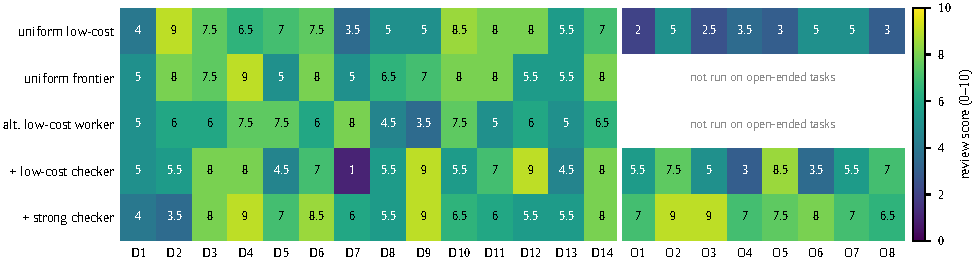
\includegraphics{fig-heatmap.pdf}
\caption{Mean review score per issue (columns; D = defect fix, O = open-ended) and configuration (rows). The uniform frontier crew and the alternative low-cost worker were not run on open-ended tasks.}
\label{fig:heatmap}
\end{figure}

{\scriptsize\setlength{\tabcolsep}{4pt}
\begin{longtable}{llccccc}\caption{Per-issue results: mean review score / cost in dollars per configuration; $^\times$ marks a candidate that at least one reviewer rejected; -- = not run.}\label{tab:perissue}\\\toprule
id & repository--issue & uniform low-cost & alt.\ worker & + low-cost chk & + strong chk & uniform frontier\\\midrule\endfirsthead
\toprule
id & repository--issue & uniform low-cost & alt.\ worker & + low-cost chk & + strong chk & uniform frontier\\\midrule\endhead
D1 & \texttt{Abhigyan-Shekhar-Waggle-mcp-635} & 4$^\times$ / 0.021 & 5 / 0.061 & 5 / 0.028 & 4 / 0.108 & 5 / 0.530\\
D2 & \texttt{Hebbian-Robotics-hflow-586} & 9 / 0.030 & 6 / 0.139 & 5.5 / 0.020 & 3.5$^\times$ / 0.024 & 8 / 0.444\\
D3 & \texttt{UKGovernmentBEIS-inspect\_ai-5295} & 7.5 / 0.022 & 6 / 0.062 & 8 / 0.022 & 8 / 0.041 & 7.5 / 0.225\\
D4 & \texttt{cubrid-lab-pycubrid-368} & 6.5 / 0.008 & 7.5 / 0.040 & 8 / 0.011 & 9 / 0.062 & 9 / 0.160\\
D5 & \texttt{fairlearn-fairlearn-1165} & 7 / 0.009 & 7.5 / 0.026 & 4.5$^\times$ / 0.014 & 7 / 0.121 & 5 / 0.153\\
D6 & \texttt{mesa-mesa-2494} & 7.5 / 0.013 & 6 / 0.029 & 7 / 0.009 & 8.5 / 0.068 & 8 / 0.198\\
D7 & \texttt{nesquena-hermes-webui-7693} & 3.5$^\times$ / 0.024 & 8 / 0.064 & 1$^\times$ / 0.033 & 6 / 0.043 & 5 / 0.563\\
D8 & \texttt{nipoppy-nipoppy-897} & 5 / 0.019 & 4.5 / 0.023 & 5.5 / 0.015 & 5.5 / 0.148 & 6.5 / 0.319\\
D9 & \texttt{openwisp-netjsonconfig-412} & 5 / 0.063 & 3.5$^\times$ / 0.081 & 9 / 0.042 & 9 / 0.057 & 7 / 0.331\\
D10 & \texttt{oxpull-django-ox-65} & 8.5 / 0.016 & 7.5 / 0.070 & 5.5$^\times$ / 0.028 & 6.5 / 0.195 & 8 / 0.234\\
D11 & \texttt{plotly-plotly.py-3065} & 8 / 0.018 & 5 / 0.055 & 7 / 0.016 & 6 / 0.107 & 8 / 0.406\\
D12 & \texttt{runtorque-torque-613} & 8 / 0.046 & 6 / 0.156 & 9 / 0.101 & 5.5$^\times$ / 0.065 & 5.5 / 0.792\\
D13 & \texttt{use-agent-os-agent-os-2882} & 5.5 / 0.014 & 5 / 0.020 & 4.5 / 0.019 & 5.5 / 0.058 & 5.5 / 0.302\\
D14 & \texttt{vedaant00-opendot-163} & 7 / 0.016 & 6.5 / 0.046 & 8 / 0.023 & 8 / 0.068 & 8 / 0.253\\
O1 & \texttt{Bouni-kicad-jlcpcb-tools-617} & 2$^\times$ / 0.098 & -- & 5.5 / 0.069 & 7 / 0.107 & --\\
O2 & \texttt{Oaklight-llm-rosetta-732} & 5$^\times$ / 0.030 & -- & 7.5 / 0.030 & 9 / 0.249 & --\\
O3 & \texttt{amaranth-lang-amaranth-987} & 2.5$^\times$ / 0.033 & -- & 5 / 0.055 & 9 / 0.085 & --\\
O4 & \texttt{apache-dolphinscheduler-sdk-python-88} & 3.5$^\times$ / 0.016 & -- & 3$^\times$ / 0.013 & 7 / 0.103 & --\\
O5 & \texttt{astropy-astropy-13539} & 3$^\times$ / 0.010 & -- & 8.5 / 0.014 & 7.5 / 0.059 & --\\
O6 & \texttt{cleder-fastkml-455} & 5$^\times$ / 0.025 & -- & 3.5$^\times$ / 0.049 & 8 / 0.086 & --\\
O7 & \texttt{gyli-PyWaffle-26} & 5$^\times$ / 0.033 & -- & 5.5 / 0.054 & 7 / 0.106 & --\\
O8 & \texttt{unit8co-darts-1112} & 3$^\times$ / 0.147 & -- & 7 / 0.076 & 6.5 / 0.139 & --\\
\bottomrule\end{longtable}
}

\clearpage
\subsection{Review protocol and agreement}
\label{app:review}
Each issue's packet contained the issue text, the base checkout, the merged pull request's diff as a reference, and every candidate diff under a random six-hex identifier; the key from identifier to configuration was stored separately and never shown. Anything that could reveal a model was stripped from the diffs. Reviewers scored resolution, correctness, code quality and risk (0--3 each), an overall score (0--10), a mergeability verdict and a one-sentence justification.

\begin{table}[h]
\centering\small
\begin{tabular}{lr}\toprule
statistic (103 doubly-reviewed candidates) & value\\\midrule
Spearman correlation, overall score & 0.88\\
Pearson correlation, overall score & 0.90\\
ICC(2,1), single rater, absolute agreement & 0.90\\
ICC(2,2), mean of two raters & 0.95\\
mean absolute difference (points) & 0.58\\
within 1 point / within 2 points & 92\% / 99\%\\
Cohen's $\kappa$, three-way mergeability & 0.77\\
Cohen's $\kappa$, mergeable vs.\ not & 0.83\\
\bottomrule\end{tabular}
\caption{Inter-reviewer agreement.}
\end{table}

\paragraph{Blind review as the endpoint.} Review measures what a maintainer would merge. A reference pull request's tests measure agreement with one particular implementation: on the 74 defect-fix candidates with a reference-test verdict, 29 changes that fail the reference tests are judged mergeable by both reviewers (the tests pin the reference's exact interface or wording), and review and reference tests disagree on 42\% of candidates overall.

\clearpage
\section{Additional plots}
\begin{figure}[h]
\centering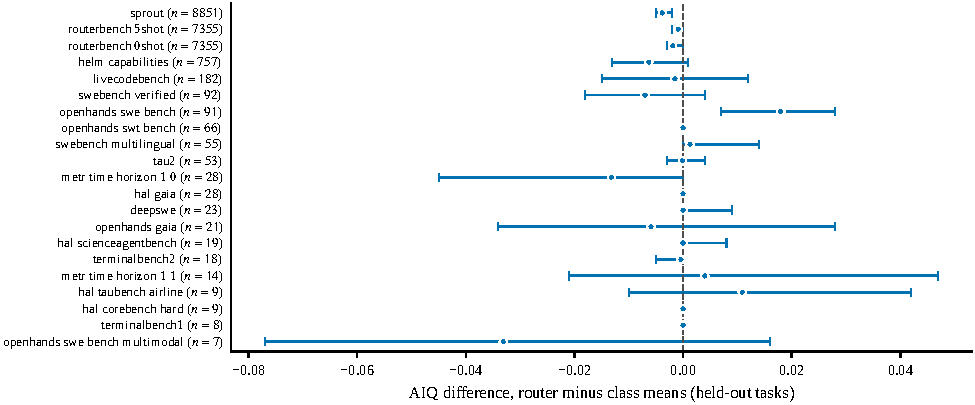
\includegraphics{fig-s1-matrix.pdf}
\caption{Per-matrix difference between the deployed router and the class-mean router on held-out tasks (S1, three seeds, paired task-bootstrap 95\% CI). Differences are within $\pm0.02$ AIQ on 20 of 21 matrices, as \cref{thm:class} predicts.}
\end{figure}

\begin{figure}[h]
\centering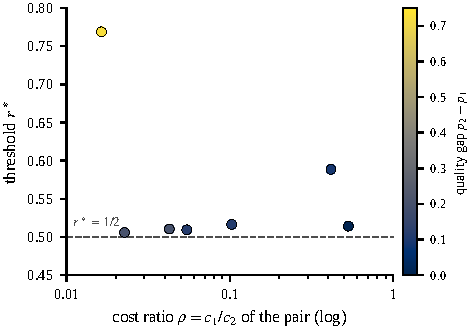
\includegraphics{fig-theory-pairs.pdf}
\caption{Threshold $r^\ast$ of \cref{thm:rstar} for pairs of DeepSWE hull configurations against the pair's cost ratio $\rho$ (log scale), coloured by the pair's quality gap $p_2-p_1$. The dashed line is $r^\ast=\tfrac12$, the limit of \cref{cor:half}; the one pair far above it has a cheap member that almost never succeeds.}
\label{fig:theory-pairs}
\end{figure}

\end{document}
